\documentclass[12pt]{scrbook}

%%%%%%%%%%%%%%%%%%%%%%%%%%%%%%%%%%%%%%%%%%%%%%%%%%%%%%%%%%
%                                                        %
% Uncomment the follwing, if you want to use pdfTeX      %
%                                                        % 
%%%%%%%%%%%%%%%%%%%%%%%%%%%%%%%%%%%%%%%%%%%%%%%%%%%%%%%%%%

\usepackage[pdftex]{graphicx}
\usepackage[pdftex,                %%% hyper-references for pdflatex
bookmarks=true,                    %%% generate bookmarks ...
bookmarksnumbered=true,            %%% ... with numbers
hypertexnames=false,               %%% needed for correct links to figures !!!
breaklinks=true,                   %%% break links if exceeding a single line
colorlinks=true,
urlcolor = blue,
citecolor = blue,
urlcolor = blue]{hyperref}

%%%%%%%%%%%%%%%%%%%%%%%%%%%%%%%%%%%%%%%%%%%%%%%%%%%%%%%%%%
%                                                        %
% Uncomment the follwing, if you want to use plain LaTeX %
%                                                        % 
%%%%%%%%%%%%%%%%%%%%%%%%%%%%%%%%%%%%%%%%%%%%%%%%%%%%%%%%%%
% \usepackage{graphicx}
% \newcommand{\href}[2]{{\tt #1}}


%%%%%%%%%%%%%%%%%%%%%%%%%%%%%%%%%%%%%%%%%%%%%%%%%%%%%%%%%%
%                                                        %
% Common section for both plain LaTeX and pdfTex         %
%                                                        % 
%%%%%%%%%%%%%%%%%%%%%%%%%%%%%%%%%%%%%%%%%%%%%%%%%%%%%%%%%%

\usepackage{a4wide}
\usepackage{times}
\usepackage{fancyhdr}
% Note: next line required to enable longtable to work.
\usepackage{longtable}

\setcounter{secnumdepth}{2}

\sloppy
% page headings

\pagestyle{fancyplain}
\renewcommand{\chaptermark}[1]{\markboth{#1}{#1}}
\renewcommand{\sectionmark}[1]{\markright{\thesection\ #1}}
\lhead[\sf\bfseries\fancyplain{}{\thepage}]{\sf\fancyplain{}{\rightmark}}
\rhead[\sf\fancyplain{}{\leftmark}]{\sf\bfseries\fancyplain{}{\thepage}}
\cfoot{}

\title{JacORB 1.4 Programming Guide}

\author{Gerald Brose, Nicolas Noffke\\
\{gerald.brose@xtradyne.com, nicolas.noffke@epost.de\}\\
\\
$$
}

\begin{document}

% uniform formatting of a command line, includes leading $
\newcommand{\cmdline}[1]{\begin{small}\noindent \texttt{\$ #1}\end{small}}

% Use these instead of writing version numbers directly, so
% version changes only have to be made in one place
\newcommand{\JacORBDir}{JacORB1\_4}
\newcommand{\JacORBVersion}{1.4.1}

\maketitle


\setlength{\parskip}{1.1ex}
\newpage
\tableofcontents

\chapter{Introduction}

This  document  gives   an  introduction  to  programming  distributed
applications with  JacORB, a free  Java object request  broker. JacORB
comes  with  full  source  code,  a couple  of  CORBA  Object  Service
implementations, and  a number of example programs.   This document is
{\it  not}   an  introduction  to   CORBA  in  general.    Please  see
\cite{Brose2001a,Siegel2000,   Vinoski1997}  for   this   purpose  and
\cite{Henning1999}  for  more  advanced  issues.  The  JacORB  version
described in this document  is JacORB \JacORBVersion. This document is
intended  to give  a few  essential hints  on how  to install  and use
JacORB, but  it will  not suffice as  either a gentle  introduction to
CORBA or a tutorial.

%%%%%%%%%%%%%%%%%%%%%%%%%%%%%%%%%%%%%%%%%%%%%%%%%%%%%%%%%%%%%%%%%%%%%%%%%%%%%%

\chapter{Installing JacORB}
\label{Ch_installing}

In this chapter  we explain how to obtain and  install JacORB and give
an overview of the package contents.

\section{Downloading JacORB}


JacORB can be downloaded as a g-zipped tar--archive or as a zip--archive
from the  JacORB home page  at
\href{http://www.jacorb.org}{http://www.jacorb.org}.

To install JacORB, just unzip  and untar (or simply unzip) the archive
somewhere.  This will result  in a new directory {\tt \JacORBDir}.
Make   sure  your   CLASSPATH  environment   variable   contains  {\tt
\JacORBDir/lib/jacorb.jar}. Extend  your search path  with
{\tt  \JacORBDir/bin}, so  that the shell scripts and batch files  for
the utilities in this directory are found.

\section{Installation}
\label{Sec_installation}

\subsection{Requirements}

JacORB requires JDK 1.2 or above properly installed on your machine.  To build
JacORB (and compile the examples) you need to have the XML--based make tool
``Ant'' installed on your machine.  Ant can be downloaded from
\href{http://jakarta.apache.org/ant}{http://jakarta.apache.org/ant}. All make
files ({\tt build.xml}) are written for this tool. To rebuild JacORB
completely, just type {\tt ant} in the installation directory.  Optionally,
you might want to do a {\tt ant clean} first.

For SSL, you need an implementation of the SSL protocol. We currently support:

\begin{enumerate}
\item IAIK's
  \footnote{\href{http://jcewww.iaik.tu-graz.ac.at}{http://jcewww.iaik.tu-graz.ac.at/}}
  implementation consisting of the crypto provider IAIK--JCE 2.5 (or higher)
  and the SSL library iSaSiLk 3.0 (or higher). Using this implementation
  allows you to access the clients authenticated certificates.
\item Sun's JSSE Reference implementation included in the JDK 1.4 and
  separately available from the Developer Connection.
\end{enumerate}

\subsection{Configuration}
\label{configuration}

JacORB has a number of configuration  options which can be set as Java
properties.  Before we will go about explaining some of the more basic
options   here,  let's  look   at  the   different  ways   of  setting
properties. Specific  options that apply, e.g.,  to the Implementation
Repository  or  the  Trading  Service  are explained  in  the  chapter
discussing these modules. There are three options for doing this.

The most  general case is in  a properties file. JacORB  looks for and
loads  a   file  called  either  {\tt   .jacorb\_properties}  or  {\tt
jacorb.properties}. The properties files will be searched in the
following places:
\begin{enumerate}
  \item in the classpath.
  \item in the home directory of the user running JacORB. This is
        obtained by calling {\tt System.getProperty( "user.home" )}.
        So if in doubt where your home directory is, write a small
        java programm that prints out this property.
  \item in the current directory.
  \item in the {\tt lib} directory of the JDK installation. The JDKs
        home directory is obtained by calling
        {\tt System.getProperty( "java.home" )}.
\end{enumerate}

The places are searched in the order presented above. If a properties
file is found, it is loaded and searching is terminated.

For  more  application--specific  properties,  you  can  pass  a  {\tt
  java.util.Properties} object to  {\tt ORB.init()} during application
  initialization. Properties set this way will override properties set
  by a properties file. The following code snippet demonstrates how to
  pass in  a {\tt Properties} object  ({\tt args} is  the String array
  containing command line arguments):

\small{
\begin{verbatim}
    java.util.Properties props = new java.util.Properties();
    props.setProperty("jacorb.implname","StandardNS");
    // use put() under Java 1.1

    org.omg.CORBA.ORB orb = org.omg.CORBA.ORB.init(args, props);
\end{verbatim}
}

The next way of specifying properties is by setting the JVMs system
properties.  These properties must be set prior to calling {\tt ORB.init()},
and will override both properties that are loaded via file and an additional
{\tt Properties} object.  System properties can also be set using the {\tt
  -D<prop name>=<prop value>} command line arg. This is a command line argument
to the java command (and not something we invented), but can be used with the
{\tt jaco} script as well. The only thing you have to take care of is that
this argument must be placed somewhere in front of the class name argument.
Anything that follows after the class name is interpreted (by {\tt java}) as a
command line argument to the class and will be visible in the {\tt args}
parameter of the classes main method.

If you want to set more than one property on the command line, you can use the
special property ``custom.props''. The value of this property has to be the
filename to a properties file, which contains the properties you want to load.
The filename is used ``as is'', and not interpreted to be relative to any
other directory as the current one. The properties contained in the specified
file will override any properties already set by the ``normal'' properties
file. As an example, imagine that you usually use plain TCP/IP connections,
but in some cases want to use SSL (see section \ref{SSL}). If you use just one
properties file, you always have to edit that if you want to switch between
SSL and plaintext connections. If you don't want to edit the properties file
all the time, you can also add every different property in the way described
in the previous paragraph, which may lead to very long commands. If you use a
custom properties file, you have all the additional properties to set in one
single file, and you only have to add one command line property, for example:

\cmdline{jaco -Dcustom.props=ssl\_props MyServer}

We are now ready to have a look at the most basic JacORB configuration
properties.  Here is an example {\tt jacorb\_properties} file:

\renewcommand{\baselinestretch}{0.9}
\small{
\begin{verbatim}
##
##  JacORB configuration options
##

########################################
#                                      #
#   Initial references configuration   #
#                                      #
########################################

#
# URLs where IORs are stored (used in orb.resolve_initial_service())
# DO EDIT these! (Only those that you are planning to use,
# of course ;-).
#
# The ORBInitRef references are created on ORB startup time. In the
# cases of the services themselves, this may lead to exceptions being
# displayed (because the services aren't up yet). These exceptions
# are handled properly and cause no harm!

#ORBInitRef.NameService=corbaloc::160.45.110.41:38693/\
#                       StandardNS/NameServer%2DPOA/_root
#ORBInitRef.NameService=file:/c:/NS_Ref
ORBInitRef.NameService=http://www.x.y.z/~user/NS_Ref
#ORBInitRef.TradingService=http://www.x.y.z/~user/TraderRef

# JacORB-specific URLs
jacorb.ImplementationRepositoryURL=http://www.x.y.z/~user/ImR_Ref
jacorb.ProxyServer.URL=http://www.x.y.z/~user/Appligator_Ref

##################################
#                                #
#   Debug output configuration   #
#                                #
##################################

# use (java) jacorb.util.CAD to generate an appropriate
# verbosity level
# 0 = off
# 1 = important messages and exceptions
# 2 = informational messages and exceptions
# >= 3 = debug-level output (may confuse the unaware user :-)
jacorb.verbosity=1

# where does output go? Terminal is default
#jacorb.logfile=LOGFILEPATH

# Whether to timestamp log entries
jacorb.log.timestamp=off

# If logging to file whether to append to existing file or overwrite
jacorb.logfile.append=off

# If jacorb.logfile.append is on, set rolling log size in kilobytes.
# A value of 0 implies no rolling log
jacorb.logfile.maxLogSize=0

# hexdump outgoing messages
jacorb.debug.dump_outgoing_messages=off

# hexdump incoming messages
jacorb.debug.dump_incoming_messages=off

##################################################
#                                                #
#    WARNING: The following properties should    #
#    only be edited by the expert user. They     #
#    can be left untouched for most cases!       #
#                                                #
##################################################

################################
#                              #
#   Basic ORB Configuration    #
#                              #
################################

# number of retries if connection cannot directly be established
jacorb.retries=5

# how many msecs. do we wait between retries
jacorb.retry_interval=500

# size of network buffers for outgoing messages
jacorb.outbuf_size=2048

# client-side timeout, set no non-zero to stop blocking
# after so many msecs.
#jacorb.connection.client_timeout=0

# max time a server keeps a connection open if nothing happens
#jacorb.connection.server_timeout=10000

#jacorb.reference_caching=off
...

#########################
#                       #
#   POA Configuration   #
#                       #
#########################

# displays a GUI monitoring tool for servers
jacorb.poa.monitoring=off

# thread pool configuration for request processing
jacorb.poa.thread_pool_max=20
jacorb.poa.thread_pool_min=5

# if set, request processing threads in thePOA
# will run at this priority. If not set or invalid,
# MAX_PRIORITY will be used.
#jacorb.poa.thread_priority=

# size of the request queue, clients will receive Corba.TRANSIENT
# exceptions if load exceeds this limit
jacorb.poa.queue_max=100
...
\end{verbatim}
}
\renewcommand{\baselinestretch}{1.0}
\small\normalsize

Configurable options  include the size of network  buffers, the number
of retries JacORB makes if a connection cannot be established, and how
long  it  shall wait  before  retrying.   The  string value  for  {\tt
ORBInitRef.NameService} is  a URL  for a resource  used to set  up the
JacORB name  server. This URL  will be used  by the ORB to  locate the
file  used to  store  the  name server's  object  reference (see  also
chapter \ref{names}).

The {\tt verbosity} option tells  JacORB how much diagnostic output it
should emit at runtime. Unless the  {\tt logfile} property is set to a
file name, diagnostic output will  be sent to the terminal. Setting the
verbosity property to 0 means don't print any, while a level of 2 is a
verbose debug mode.   Level 1 will emit some  information, e.g.  about
connections  being  opened,  accepted  and  closed.  If  you  like  to
selectively  suppress  specific  output  you  can  use  the  tool  {\tt
jacorb.util.CAD} to generate a special verbosity level.

The  {\tt jacorb.poa.monitoring} property  determines whether  the POA
should bring up a monitoring GUI  for servers that let you examine the
dynamic behavior of  your POA, e.g.  how long  the request queue gets
and whether your thread pool is  big enough.  Also, this tool lets you
change the  state of a POA,  e.g. from {\it active}  to {\it holding}.
Please see chapter \ref{POA} on the POA for more details.

You can now test your installation  by typing {\tt ant} in one of the
subdirectories of the {\tt demo/} directory which contains a number of
examples for using JacORB.

%%%%%%%%%%%%%%%%%%%%%%%%%%%%%%%%%%%%%%%%%%%%%%%%%%%%%%%%%%%%%%%%%%%%%%%%%%%%%%

\chapter{Getting Started}
\label{start}

Before we  explain an example  in detail, we  will have a look  at the
general process  of developing  CORBA applications with  JacORB. We'll
follow this roadmap when working through the example.  The example can
be found in  {\tt demo/grid} which also contains a  build file so that
the development  steps do  not have to  be carried out  manually every
time.  Still, you should know what is going on.

As this document gives only a short introduction to JacORB programming
and does not cover all the details of CORBA IDL, we recommend that you
also look at  the other examples in the  {\tt demo/} directory.  These
are organized so as to show how the different aspects of CORBA IDL can
be used with JacORB.

\section{JacORB development: an overview}

The steps we will generally have to take are:

\begin{enumerate}
    \item  write an IDL specification.
    \item  compile this specification with the IDL compiler to generate Java classes.
    \item write an implementation for the interface generated in step 2
    \item  write a ``Main'' class that instantiates the server implementation
        and registers it with the ORB
    \item  write a client class that retrieves a reference to the server object.
\end{enumerate}


\section{IDL specifications}

Our example uses a simple server the definition of which should be
clear if you know IDL. Its interface is given in {\tt server.idl}. All
the source code for this example can be found in {\tt \JacORBDir/demo/grid}.

{\small
\begin{verbatim}
// server.idl
// IDL definition of a 2-D grid:
module demo
{
  module grid
  {
    interface MyServer
    {
        typedef fixed <5,2> fixedT;

        readonly attribute short height;  // height of the grid
        readonly attribute short width;   // width of the grid

        // set the element [n,m] of the grid, to value:
        void set(in short n, in short m, in fixedT value);

        // return element [n,m] of the grid:
        fixedT get(in short n, in short m);

        exception MyException
        {
            string why;
        };

        short opWithException() raises( MyException );
    };
  };
};
\end{verbatim}
}

\section{Generating Java classes}

Feeding this file into the IDL compiler

\cmdline{idl -d ../..  server.idl}

produces a number of Java  classes that represent the IDL definitions.
This is  done according to a  set of rules known  as the IDL--to--Java
language mapping as standardized by  the OMG. If you are interested in
the details of the language mapping, i.e. which IDL language construct
is  mapped  to  which  Java  language construct,  please  consult  the
specifications available from  {\tt www.omg.org}. The language mapping
used by the JacORB IDL compiler is the one defined in CORBA 2.3 and is
explained in detail in  \cite{Brose2001a}. For practical usage, please
consult the examples in the {\tt demo} directory.

The most important Java classes  generated by the IDL compiler are the
interfaces {\tt  MyServer} and {\tt MyServerOperations}  plus the stub
and  skeleton   files  {\tt  \_MyServerStub,   MyServerPOA}  and  {\tt
MyServerPOATie}.  We will  use these classes in the  client and server
as  well as  in the  implementation  of the  grid's functionality  and
explain each in turn.

Note that the IDL compiler  will produce a directory structure for the
generated code  that corresponds  to the module  structure in  the IDL
file, so it would have  produced a subdirectory {\tt demo/grid} in the
current  directory  had we  not  directed  it  to put  this  directory
structure  to {\tt  ../..} by  using the  compiler's {\tt  -d} switch.
Where to  put the source  files for generated  classes is a  matter of
taste.  Some people  prefer to have everything in  one place (as using
the {\tt  -d} option in  this way achieves),  others like to  have one
subdirectory for the generated source  code and another for the output
of the Java compiler, i.e. for the {\tt .class} files.


\section{Implementing the interface}

Let's try  to actually provide an implementation  of the functionality
promised by  the interface. The class which  implements that interface
is called {\tt gridImpl}.   Apart from providing a Java implementation
for the operations listed in the IDL interface, it has to inherit from
a generated class that both  defines the Java type that represents the
IDL type {\tt MyServer} and contains the code needed to receive remote
invocations and return results to  remote callers.  This class is {\tt
MyServerPOA}.

You might have noticed that this approach is impractical in situations
where your  implementation class needs to inherit  from other classes.
As  Java only has  single inheritance  for implementations,  you would
have  to use  an alternative  approach ---  the  ``tie''--approach ---
here. The tie approach will be explained later.

Here is  the Java code for  the grid implementation. It  uses the Java
library  class  {\tt  java.math.BigDecimal}  for  values  of  the  IDL
fixed--point type {\tt fixedT}:

\small{
\begin{verbatim}
package demo.grid;

/**
 * A very simple implementation of a 2-D grid
 */

import demo.grid.MyServerPackage.MyException;

public class gridImpl
    extends MyServerPOA
{
    protected short height = 31;
    protected short width = 14;
    protected java.math.BigDecimal[][] mygrid;

    public gridImpl()
    {
        mygrid = new java.math.BigDecimal[height][width];
        for( short h = 0; h < height; h++ )
        {
            for( short w = 0; w < width; w++ )
            {
                mygrid[h][w] = new java.math.BigDecimal("0.21");
            }
        }
    }

    public java.math.BigDecimal get(short n, short m)
    {
        if( ( n <= height ) && ( m <= width ) )
            return mygrid[n][m];
        else
            return new java.math.BigDecimal("0.01");
    }

    public short height()
    {
        return height;
    }

    public void set(short n, short m, java.math.BigDecimal value)
    {
        if( ( n <= height ) && ( m <= width ) )
            mygrid[n][m] = value;
    }

    public short width()
    {
        return width;
    }

    public short opWithException()
        throws demo.grid.MyServerPackage.MyException
    {
        throw new demo.grid.MyServerPackage.MyException("This is only a test exception, no harm done :-)");
    }
}
\end{verbatim}
}

\section{Writing the Server}

To actually instantiate a {\tt  gridImpl} object which can be accessed
remotely  as  a CORBA  object  of type  {\tt  MyServer},  you have  to
instantiate it  in a main method  of some other class  and register it
with a  component of the CORBA  architecture known as  the {\it Object
Adapter}. Here is  the class {\tt Server} which  does all that is
necessary to  activate a  CORBA object of  type {\tt MyServer}  from a
Java {\tt gridImpl} object:

\small{
\begin{verbatim}
package demo.grid;

import java.io.*;
import org.omg.CosNaming.*;

public class Server
{
    public static void main( String[] args )
    {
        org.omg.CORBA.ORB orb = org.omg.CORBA.ORB.init(args, null);
        try
        {
            org.omg.PortableServer.POA poa =
                org.omg.PortableServer.POAHelper.narrow(
                     orb.resolve_initial_references("RootPOA"));

            poa.the_POAManager().activate();

            org.omg.CORBA.Object o = poa.servant_to_reference(new gridImpl());

            if( args.length == 1 )
            {
                // write the object reference to args[0]

                PrintWriter ps = new PrintWriter(
                                    new FileOutputStream(
                                       new File( args[0] )));
                ps.println( orb.object_to_string( o ) );
                ps.close();
            }
            else
            {
                // register with the naming service

                NamingContextExt nc =
                     NamingContextExtHelper.narrow(
                        orb.resolve_initial_references("NameService"));
                nc.bind( nc.to_name("grid.example"), o);
            }
        }
        catch ( Exception e )
        {
            e.printStackTrace();
        }
        orb.run();
    }
}
\end{verbatim}
}

After initializing the ORB we need to obtain a reference to the object
adapter --- the POA --- by asking  the ORB for it. The ORB knows about
a few initial references that can be retrieved using simple names like
``RootPOA''. The returned object is  an untyped reference of type {\tt
CORBA.Object} and thus needs to  be narrowed to the correct type using
a static  method {\tt narrow()}  in the helper  class for the  type in
question. We now  have to activate the POA because  any POA is created
in  ``holding''   state  in  which   it  does  not   process  incoming
requests.  After  calling {\tt  activate()}  on  the POA's  POAManager
object, the POA is in an active state and can now be asked to create a
CORBA  object  reference  from a  Java  object  also  know as  a  {\tt
Servant}.

In order to make the newly created CORBA object accessible, we have to
make its  object reference  available. This is  done using  a publicly
accessible directory  service, the naming  server. A reference  to the
naming      service     is      obtained      by     calling      {\tt
orb.resolve\_initial\_references("NameService")}   on   the  ORB   and
narrowing the reference using the {\tt narrow()} method found in class
{\tt org.omg.CosNaming.NamingContextExtHelper}.  Having done this, you
should call the  {\tt bind()} operation on the  name server.  The name
for the object which has to be supplied as an argument to {\tt bind()}
is not simply a string. Rather, you need to provide a sequence of {\tt
CosNaming.NameComponent}s that represent the  name. In the example, we
chose to use an extended Name Server interface that provides us with a
more convenient conversion operation from strings to Names.


\section{Writing a client}

Finally, let's have a look at the client class which invokes the
server operations:

\small{
\begin{verbatim}
package demo.grid;

import org.omg.CosNaming.*;

public class Client
{
   public static void main(String args[])
   {
       try
       {
           MyServer grid;
           org.omg.CORBA.ORB orb = org.omg.CORBA.ORB.init(args,null);

           if(args.length==1 )
           {
               // args[0] is an IOR-string
               grid = MyServerHelper.narrow(orb.string_to_object(args[0]));
           }
           else
           {
               NamingContextExt nc =
                   NamingContextExtHelper.narrow(
                      orb.resolve_initial_references("NameService"));

               grid = MyServerHelper.narrow(
                         nc.resolve(nc.to_name("grid.example")));
            }

            short x = grid.height();
            System.out.println("Height = " + x);

            short y = grid.width();
            System.out.println("Width = " + y);

            x -= 1;
            y -= 1;

            System.out.println("Old value at (" + x + "," + y +"): " +
                               grid.get( x,y));

            System.out.println("Setting (" + x + "," + y +") to 470.11");

            grid.set( x, y, new java.math.BigDecimal("470.11"));

            System.out.println("New value at (" + x + "," + y +"): " +
                               grid.get( x,y));

           try
           {
               grid.opWithException();
           }
           catch (jacorb.demo.grid.MyServerPackage.MyException ex)
           {
               System.out.println("MyException, reason: " + ex.why);
           }
       }
       catch (Exception e)
       {
           e.printStackTrace();
       }
   }
}
\end{verbatim}
}

After  initializing the  ORB, the  client obtains  a reference  to the
``grid''  service by locating  the reference  using the  name service.
Again, resolving the name is done by getting a reference to the naming
service                 by                 calling                {\tt
orb.resolve\_initial\_references("NameService")} and querying the name
server for  the {\tt "grid"}  object by calling {\tt  resolve()}.  The
argument  to  the  resolve  operation  is, again,  a  string  that  is
converted to  a Name. The result  is an object reference  of type {\tt
org.omg.CORBA.Object}  which has  to be  narrowed to  the type  we are
expecting, i.e. {\tt MyServer}.

After compiling everything we're now  ready to actually run the server
and the  client on  different (virtual) machines.  Make sure  the name
server is running before starting  either the server or the client. If
it isn't, type something like:

\cmdline{ns /home/me/public\_html/NS\_Ref}

where  {\tt /home/me/public\_html/NS\_Ref}  is the  name of  a locally
writable file  which can be  read by using  the URL given in  both the
remote client and  server code. (This is to  avoid using a well--known
address for  the name server,  so both client  and server look  up the
location of the  name server via the URL and  later communicate with it
directly.)

You can now launch the server:

\cmdline{jaco demo.grid.Server}

The client can be invoked on any machine you like:

\cmdline{jaco demo.grid.Client}

Running the  client after starting  the server produces  the following
output on your terminal:

\begin{verbatim}
Height = 31
Width = 14
Old value at (30,13): 0.21
Setting (30,13) to 470.11
New value at (30,13): 470.11
MyException, reason: This is only a test exception, no harm done :-)
done.
\end{verbatim}

\subsection{The Tie Approach}

If your implementation class cannot inherit from the generated servant
class  {\tt  MyServerPOA} because,  e.g.,  you  need  to inherit  from
another  base class,  you can  use the  tie approach.  Put  simply, it
replaces  inheritance by  delegation. Instead  of inheriting  from the
generated  base  class, your  implementation  needs  to implement  the
generated {\em operations interface} {\tt MyServerOperations}:

\begin{verbatim}
package demo.grid;

import demo.grid.MyServerPackage.MyException;

public class gridOperationsImpl
    implements MyServerOperations
{
...
}
\end{verbatim}

Your server is then written as follows:

\begin{verbatim}
package demo.grid;

import java.io.*;
import org.omg.CosNaming.*;

public class TieServer
{
    public static void main( String[] args )
    {
        org.omg.CORBA.ORB orb =
            org.omg.CORBA.ORB.init(args, null);
        try
        {
            org.omg.PortableServer.POA poa =
                org.omg.PortableServer.POAHelper.narrow(
                     orb.resolve_initial_references("RootPOA"));

            // use the operations implementation and wrap it in
            // a tie object

            org.omg.CORBA.Object o =
                poa.servant_to_reference(
                     new MyServerPOATie( new gridOperationsImpl()) );

            poa.the_POAManager().activate();

            if( args.length == 1 )
            {
                // write the object reference to args[0]

                PrintWriter ps = new PrintWriter(
                    new FileOutputStream(new File( args[0] )));
                ps.println( orb.object_to_string( o ) );
                ps.close();
            }
            else
            {
                NamingContextExt nc =
                     NamingContextExtHelper.narrow(
                        orb.resolve_initial_references("NameService"));
                NameComponent [] name = new NameComponent[1];
                name[0] = new NameComponent("grid", "whatever");
                nc.bind( name, o );
            }
        }
        catch ( Exception e )
        {
            e.printStackTrace();
        }
        orb.run();
    }
}
\end{verbatim}




%%%%%%%%%%%%%%%%%%%%%%%%%%%%%%%%%%%%%%%%%%%%%%%%%%%%%%%%%%%%%%%%%%%%%%%%%%%%%%

\chapter{The JacORB Name Service}
\label{names}

Name  servers  are used  to  locate  objects  using a  human--readable
reference (their  name) rather than  a machine or network  address. If
objects providing  a certain service  are looked up using  the service
name, their  clients are  decoupled from the  actual locations  of the
objects that provide  this service.  The binding from  name to service
can be changed without the clients needing to know.

JacORB provides an implementation of the OMG's Interoperable Naming
Service (INS) which supports binding names to object references and to
lookup object references using these names.  It also allows clients to
easily convert names to strings and vice versa.  The JacORB name
service comprises two components: the name server program, and a set
of interfaces and classes used to access the service.


One word of caution about using JDK 1.2 with the JacORB naming service: JDK
1.2 comes with a couple of outdated and apparently buggy naming service
classes that do not work properly with JacORB. To avoid having these classes
loaded and used inadvertently, please make sure that you always use the {\tt
  NamingContextExt} interface rather than the plain {\tt NamingContext}
interface in your code. Otherwise, you will see your application receive null
pointer or other exceptions.

\section{Running the Name Server}

The JacORB  name server is a  process that needs to  be started before
the name service can be accessed by programs. Starting the name server
is done by typing on the command line either simply

\cmdline{ns [<ior filename>][-p port] [-t <timeout>]}

You can also start the Java interpreter explicitly by typing

\cmdline{jaco jacorb.naming.NameServer [<filename>][-p port] [-t <timeout>]}

In the example

\cmdline{ns /home/me/public\_html/NS\_Ref}

we direct the name server process to write location information (its
own object reference) to the file {\tt /home/me/public\_html/NS\_Ref}.
A client--side ORB uses this file to locate the name server process.
The client--side ORB does not, however, need to be able to access the file through a
local or shared file system because  the file is read as a
 resource by using a URL pointing to it.  This implies that the
name server log file is accessible through a URL in the first place,
i.e., that you know of a web server in your domain which can answer
HTTP request to read the file.

The advantage of this approach is  that clients do not need to rely on
a hard--coded well known port  and that the name server is immediately
available world--wide  if the URL uses  HTTP. If you  want to restrict
name server visibility  to your domain (assuming that  the log file is
on a shared  file system accessible throughout your  domain) or you do
not have  access to a  web server, you  can use file URLs  rather than
HTTP URLs,  i.e. the URL pointing  to your name server  log file would
looks like

\noindent{\tt file:/home/brose/public\_html/NS\_Ref}

rather than

\noindent\verb+http://www.inf.fu-berlin.de/~brose/NS_Ref+

Specifying file URLs is also useful is clients and servers are run on
a single machine that may have no network connection at all. Please
note that the overhead of using HTTP is only incurred once --- when
the clients first locate the name server.  Subsequent requests will
use standard CORBA operation invocations which means they will be IIOP
requests (over TCP). In JacORB 1.4, the file name argument was made
optional because the JacORB 1.4 name server also answers requests that
are made using simplified corbaloc: URLs of the form {\tt
  corbaloc::ip-address:port/NameService}. This means that all you need
to know to construct an object reference to your name service is the
IP address of the machine and the port number  the server process is
listening on (the one specified using {\tt -p}).

The name server stores its  internal state, i.e., the name bindings in
its context,  in files  in the current  directory unless  the property
{\tt jacorb.naming.db\_dir} is set to a different directory name. This
saving is done  when the server goes down  regularly, i.e. killing the
server  with CTRL-C  will result  in loss  of data.   The  server will
restore state from its files if any files exist and are non--empty.

The second  parameter is a port number on which you want the name
service to listen for incoming requests. If this parameter is not
set, the name server will come up on the first free port it is
provided with by the operating system. The port number can also be set
using specific properties in the properties file, but the -p switch
was added merely for convenience.

The last  parameter is a time--out  value in msecs. If  this value is
set, the name server will shut down after the specified amount of time
and save  its state. This is  useful if the name  server is registered
with  the  Implementation Repository  and  can  thus  be restarted  on
demand.

\subsection*{Configuring a Default Context}

Configuring a naming context (i.e. a name server) as the ORB's default
or root context is done by  simply writing the URL that points to this
server's    bootstrap    file   to    the    properties   file    {\tt
.jacorb\_properties}.  Alternatively,  you can  set this file  name in
the property {\tt ORBInitRef.NameService} either on the command line or
within the application  as described in \ref{Sec_installation}.  After
the default  context has thus  been configured, all operations  on the
NamingContextExt  object  that  was   retrieved  by  a  call  to  {\tt
orb.resolve\_initial\_references("NameService")}   will  go   to  that
server  ---  provided  it's  running  or  can  be  started  using  the
Implementation Repository.

\section{Accessing the Name Service}

The  JacORB name  service is accessed using  the standard  CORBA
defined  interface:

\small{
\begin{verbatim}
   // get a reference to the naming service
   ORB orb = ORB.init(args, null);
   org.omg.CORBA.Object o = orb.resolve_initial_references("NameService")
   NamingContextExt nc = NamingContextExtHelper.narrow( o );

   // look up an object
   server s = serverHelper.narrow( nc.resolve(nc.to_name("server.service")) );
\end{verbatim}
}

Before an object  can be looked up, you need a  reference to the ORB's
name service. The standard way  of obtaining this reference is to call
{\tt orb.resolve\_initial\_\-referen\-ces("Name\-Service")}.  In calls using
the  standard,  extended  name  service interface,  object  names  are
represented as  arrays of {\tt NameComponent}s rather  than as strings
in  order to  allow  for  structured names.   Therefore,  you have  to
construct such an  array and specify that the  name's name is "server"
and    that    it    is    of   kind    ``service''    (rather    than
``context'').    Alternatively,    you    can   convert    a    string
``server.service''  to a  name by  calling the  {\tt NamingContextExt}
interface's {\tt to\_name()} operation, as shown above.

Now,  we can  look up  the object  by calling  {\tt resolve()}  on the
naming context, supplying the array as an argument.

\section{Constructing Hierarchies of Name Spaces}

Like directories in a file system, name spaces or contexts can contain
other contexts  to allow hierarchical structuring instead  of a simple
flat name  space. The  components of a  structured name for  an object
thus  form a path  of names,  with the  innermost name  space directly
containing the  name binding for the  object. This can  very easily be
done using {\tt NameManager} but can also be explicitly coded.

A new naming context within  an enclosing context can be created using
either   {\tt  new\_context()}   or  {\tt   bind\_new\_context()}.  The
following code snippet requests a naming context to create an inner or
subcontext using a given name and return a reference to it:
\small{\begin{verbatim}
   // get a reference to the naming service
   ORB orb = ORB.init();
   org.omg.CORBA.Object o =
      orb.resolve_initial_references("NameService");
   NamingContextExt rootContext =
      NamingContextExtHelper.narrow( o );

   // look up an object
   NameComponent[] name = new NameComponent[1];
   name[0] = new NameComponent("sub","context");
   NamingContextExt subContext =
     NamingContextExtHelper.narrow( rootContext.bind_new_context( name ));
\end{verbatim}}

Please  note   that  the  JacORB  naming  service   always  uses  {\tt
NamingContextExt} objects internally,  even if the operation signature
indicates {\tt  NamingContext} objects.  This is  necessary because of
the limitations  with JDK  1.2 as explained  at the beginning  of this
section.

\section{NameManager --- A simple GUI front-end to the Naming Service}

The graphical front-end to the name service can be started by simply calling

\cmdline{nmg}

The GUI front-end will simply look up the default context and display
its contents. Figure \ref{fig:nameManager} gives a screen shot.

\bigskip
\begin{figure}[htb]
  \begin{center}
    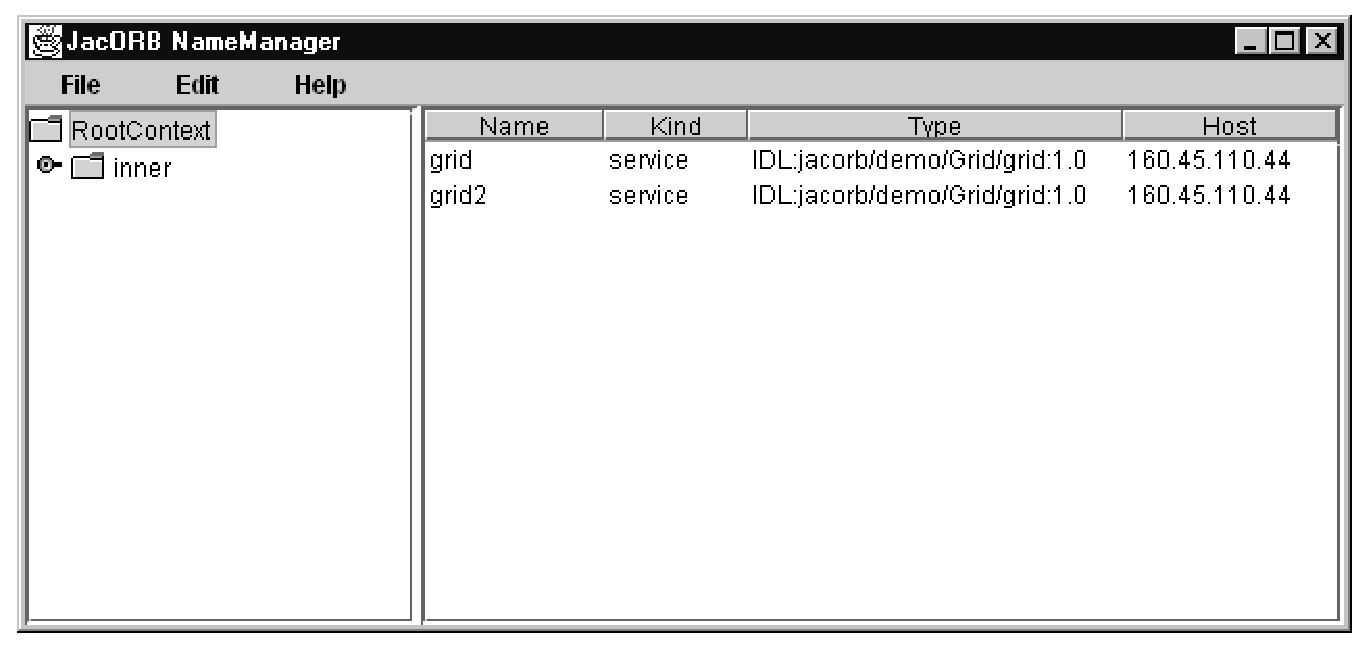
\includegraphics[width=10cm]{Nmgr1}
  \end{center}
\caption{NameManager Screenshot}
\label{fig:nameManager}
\end{figure}

NameManager has menus  that let you unbind names  and create or delete
naming contexts within the root context. Creating a nested name space,
e.g., can be done by selecting the {\tt RootContext} and bringing up a
context  by clicking  the right  mouse button.  After  selecting ``new
context'' from that menu, you will be  prompted to enter a name for the
new, nested context.


%%%%%%%%%%%%%%%%%%%%%%%%%%%%%%%%%%%%%%%%%%%%%%%%%%%%%%%%%%%%%%%%%%%%%%%%%%%%%%

\chapter{The server side: POA, Threads}
\label{POA}

This  chapter   describes  the   facilities  offered  by   JacORB  for
controlling  how servers are  started and  executed. These  include an
activation daemon, the Portable Object Adapter (POA), and threading.

This chapter gives only a very superficial introduction to the POA.  A
thorough explanation of how the POA can be used in different settings and of
the different policies and strategies it offers is beyond our scope here, but
can be found in \cite{Brose2001a}.  Other references that explain the POA are
\cite{Henning1999, Vinoski1998}.  More in--depth treatment in C++ can be found
in the various C++-Report Columns on the POA by Doug Schmidt and Steve
Vinoski.  These articles are available at
\href{http://www.cs.wustl.edu/~schmidt/report-doc.html}{http://www.cs.wustl.edu/~schmidt/report-doc.html}.
The ultimate reference, of course, is the CORBA specification.

\section{POA}

The POA provides a comprehensive set of interfaces for managing object
references and servants. The code  written using the POA interfaces is
now portable across ORB implementations  and has the same semantics in
every ORB that is compliant to CORBA 2.2 or above.

The POA defines standard interfaces to do the following:
\begin{itemize}
\item Map an object reference to a servant that implements that object
\item Allow transparent activation of objects
\item Associate policy information with objects
\item  Make a  CORBA  object persistent  over  several server  process
lifetimes
\end{itemize}

In the POA specification, the use of pseudo-IDL has been deprecated in
favor  of an approach  that uses  ordinary IDL,  which is  mapped into
programming languages using the  standard language mappings, but which
is  locality constrained.  This means  that references  to  objects of
these types may not be passed outside of a server's address space. The
POA  interface  itself  is  one  example of  a  locality--constrained
interface.

The  object adapter  is that  part of  CORBA that  is  responsible for
creating CORBA  objects and  object references and  --- with  a little
help  from  skeletons ---  dispatching  operation  requests to  actual
object  implementations.   In  cooperation  with   the  Implementation
Repository  it can also  activate objects,  i.e. start  processes with
programs that provide implementations for CORBA objects.

\section{Threads}

JacORB  currently  offers  one   server--side  thread  model.  The  POA
responsible for a given request will obtain a request processor thread
from  a central  thread pool.  The pool  has a  certain size  which is
always between the maximum and  minimum value configure by setting the
properties     {\tt     jacorb.poa.thread\_pool\_max}     and     {\tt
jacorb.poa.thread\_pool\_min}.

When a  request arrives and  the pool is  found to contain  no threads
because all  existing threads are  active, new threads may  be started
until     the    total    number     of    threads     reaches    {\tt
jacorb.poa.thread\_pool\_max}. Otherwise,  request processing is blocked
until a  thread is returned to  the pool. Upon  returning threads that
have  finished processing a  request to  the pool,  it must  be decided
whether  the  thread  should  actually   remain  in  the  pool  or  be
destroyed. If the current pool  size is above the minimum, a processor
thread will not be out into the pool again. Thus, the pool size always
oscillates between max and min.

Setting {\tt min} to a value  greater than one means keeping a certain
number  of   threads  ready  to  service   incoming  requests  without
delay. This is  especially useful if you now  that requests are likely
to come  in in a bursty fashion.  Limiting the pool size  to a certain
maximum  is  done to  prevent  servers  from  occupying all  available
resources.

Request  processor   threads  usually   run  at  the   highest  thread
priority. It is possible to influence thread priorities by setting the
property  {\tt jacorb.poa.thread\_priority} to  a value  between Java's
Thread.MIN\_PRIORITY and Thread.MAX\_PRIORITY. If the configured priority
value  is  invalid JacORB  will  assign  maximum  priority to  request
processing threads.




%%%%%%%%%%%%%%%%%%%%%%%%%%%%%%%%%%%%%%%%%%%%%%%%%%%%%%%%%%%%%%%%%%%%%%%%%%%%%%
\chapter{Implementation Repository}
\label{Ch_Imr}

\begin{quote}
``...  it is  very easy to be blinded to  the essential uselessness of
them by  the sense of achievement you  get from getting it  to work at
all.  In other  words --- and that is a  rock-solid principle on which
the whole of the Corporation's Galaxywide success is founded --- their
fundamental design  flaws are  completely hidden by  their superficial
design flaws.''

             D. Adams: So Long and Thanks for all the Fish
\end{quote}

The Implementation Repository is not, as its name suggests, a database
of  implementations.   Rather,  it  contains information  about  where
requests  to specific  CORBA objects  have  to be  redirected and  how
implementations  can be  transparently  instantiated if,  for a  given
request  to   an  object,  none  is   reachable.   ``Instantiating  an
implementation'' means starting a server program that hosts the target
object.  In  this  chapter  we  give  a brief  overview  and  a  short
introduction  on how to  use the  Implementation Repository.  For more
details please see \cite{Henning1999}.

\section{Overview}

Basically, the  Implementation Repository (ImR) is  an indirection for
requests  using  persistent  object  references. A  persistent  object
reference is one that was created  by a POA with a PERSISTENT lifespan
policy. This means that the lifetime of the object is longer than that
of its creating POA.   Using the Implementation Repository for objects
the lifetime  of which does not exceed  the life time of  its POA does
not make sense  as the main function of  the Implementation Repository
is to take care that such  a process exists when requests are made ---
and to start one if necessary.

To fulfill this function, the ImR  has to be involved in every request
to ``persistent  objects''.  This is achieved  by rewriting persistent
object  references to  contain {\em  not}  the address  of its  server
process but  the address  of the ImR.   Thus, requests  will initially
reach the ImR and not the actual server --- which may not exist at the
time of the request. If such a request arrives at the ImR, it looks up
the  server information  in its  internal tables  to determine  if the
target object is reachable or not.  In the latter case, the ImR has to
have  information  about how  an  appropriate  server  process can  be
started.   After   starting  this   server,  the  client   receives  a
LOCATION\_FORWARD  exception  from  the  ImR.  This  exception,  which
contains a new  object reference to the actual  server process now, is
handled by its runtime system  transparently.  As a result, the client
will automatically  reissue its request  using the new  reference, now
addressing the target directly.

\section{Using the JacORB Implementation Repository}

The  JacORB   Implementation  Repository  consists   of  two  separate
components:  a repository  process which  need  only exist  once in  a
domain, and  process startup daemons,  which must be present  on every
host that is  to start processes. Note that none  of this machinery is
necessary for processes that host  objects with a TRANSIENT life time,
such as used by the RootPOA.

First of all, the central repository process (which we will call ImR
in the following) must be started:

\cmdline{imr [-n] [-p <port>] [-i <ior\_file>][-f <file>][-b <file>] [-a]}

The   ImR   is  located   using   the   configuration  property   {\tt
ORBInitRef.ImplementationRepository}.  This property  must be set such
that  a  http  connection  can  be  made and  the  ImR's  IOR  can  be
read. Next, startup  daemons must be created on  selected hosts. To do
this, the following command must is issued on each host:

\cmdline{imr\_ssd}

When a startup  daemon is created, it contacts  the central ImR.

To register  a program such that  the ImR can start  it, the following
command is used (on any machine that can reach the ImR):

\cmdline{imr\_mg add "AServerName" -c "jaco MyServer"}

The {\tt imr\_mg} command is the  generic way of telling the ImR to do
something. It  needs another command  parameter, such as {\tt  add} in
this case. To add a server to the ImR, an {\em implementation name} is
needed. Here, it is {\tt  "AServerName"}.  If the host were the server
should be  restarted is not the  local one, use the  {\tt -h hostname}
option.  Finally, the  ImR needs to know how to  start the server. The
string {\tt "jaco  MyServer"} tells it how. The  format of this string
is simply such  that the server daemon can execute  it (using the Java
API call  {\tt exec()}), i.e.  it  must be intelligible  to the target
host's operating system.   For a Windows machine, this  could, e.g. be
{\tt "start jaco MyServer"} to have the server run in its own terminal
window, under Unix  the same can be achieved with  {\tt "xterm -e jaco
MyServer"}.

The startup  command is a  string that is  passed as the  {\em single}
argument to javas {\tt Runtime.exec()} method, without interpreting it
or adding  anything. Since {\tt  Runtime.exec()} has system--dependent
behaviour, the startup string has to reflect that. While for most unix
systems  it  is  sufficient  to  avoid shell--expansions  like  *  and
\verb+~+,  windows--based  systems  do   not  pass  the  string  to  a
commandline interpreter so a simple {\tt jaco MyServer} will fail even
if it works if directly typed in at the dos prompt. Therefore you have
to  ``wrap'' the  core  startup command  in  a call  to a  commandline
interpreter. On NT the following startup command will do the job: {\tt
cmd /c "jaco MyServer"}.  Please keep in mind that if you use the {\tt
imr\_mg} command  to set the startup  command, you have  to escape the
quotes so they appear inside of the resulting string.

If you don't  intend to have your server  automatically started by the
ImR     you      can     also     set      the     property     ``{\tt
jacorb.imr.allow\_auto\_register}'' or use the  {\tt -a} switch of the
ImR  process. If  this property  is  set, the  ImR will  automatically
create a new  entry for a server on POA activation,  if the server has
not been registered previously. In this case you don't have to use the
ImR Manager to register your server.

For a client program to be  able to issue requests, it needs an object
reference.  Up to  this  point,  we haven't  said  anything about  how
persistent object  references come into  existence. Reference creation
happens as usual, i.e. in the server application one of the respective
operations  on a  POA is  called.  For a  reference to  be created  as
``persistent'',  the POA  must  have been  created  with a  PERSISTENT
lifespan policy. This is done as in the following code snippet:

\small{
\begin{verbatim}
    /* init ORB and root POA */
    orb = org.omg.CORBA.ORB.init(args, props);
    org.omg.PortableServer.POA rootPOA =
        org.omg.PortableServer.POAHelper.narrow(
                        orb.resolve_initial_references("RootPOA"));

    /* create policies  */

    org.omg.CORBA.Policy [] policies = new org.omg.CORBA.Policy[2];
    policies[0] = rootPOA.create_id_assignment_policy(
                                IdAssignmentPolicyValue.USER_ID);
    policies[1] = rootPOA.create_lifespan_policy(
                                LifespanPolicyValue.PERSISTENT);

    /* create POA */

    POA myPOA = rootPOA.create_POA("XYZPOA",
                                rootPOA.the_POAManager(), policies);

    /* activate POAs */
    poa.the_POAManager().activate();

\end{verbatim}
}

(Note that in general the  id assignment policy will be {\tt USER\_ID}
for a POA with persistent object references because this id will often
be a key into  a database where the object state is  stored). If a POA
is created with this lifespan policy and the ORB property ``use\_imr''
is set, the ORB will try to  notify the ImR about this fact so the ImR
knows it doesn't need to start  a new process for requests that target
objects on this  POA.  To set the ORB policy,  simply set the property
{\tt  jacorb.use\_imr=on}.   The   ORB  uses  another  property,  {\tt
jacorb.implname}, as  a parameter for the  notification, i.e.~it tells
the  ImR  that a  process  using this  property's  value  as its  {\em
implementation name} is present. If  the server is registered with the
ImR, this property value has  to match the implementation name that is
used when registering.

The application  can set  these properties on  the command  line using
{\tt java -Djacorb.implname=MyName}, or in the code like this:

\small{
\begin{verbatim}
    /* create and set properties */
    java.util.Properties props = new java.util.Properties();
    props.setProperty("jacorb.use_imr","on");
    props.setProperty("jacorb.implname","MyName");

    /* init ORB  */
    orb = org.omg.CORBA.ORB.init(args, props);
\end{verbatim}
}

There are a few things  you have to consider especially when restoring
object state  at startup time or  saving the state of  your objects on
shutdown. It is important that, at startup time, object initialization
is complete when the object  is activated because from this instant on
operation calls  may come  in. The repository  knows about  the server
when the  first POA with  a PERSISTENT lifespan policy  registers, but
does not  forward object  references to clients  before the  object is
actually reachable. (Another, unreliable way to handle this problem is
to  increase the {\tt  jacorb.imr.object\_activation\_sleep} property,
so the repository waits longer for the object to become ready again.)

When the server shuts down,  it is equally important that object state
is saved by the time the last POA in the server goes down because from
this moment  the Implementation Repository regards the  server as down
and will start a new one upon requests.  Thus, a server implementor is
responsible for avoiding reader/writer problems between servers trying
to store and  restore the object state.  (One way of  doing this is to
use POA  managers to set  a POA to  holding while saving state  and to
inactive when done.)

Please keep in mind  that even if you don't have to  save the state of
your objects  on server shutdown  you {\em must} deactivate  your POAs
prior   to   exiting   your    process   (or   at   least   use   {\tt
orb.shutdown(\dots)} which  includes POA deactivation).  Otherwise the
ImR keeps the  server as active and will return  invalid IORs. In case
of  a  server crash  you  can either notify the ImR manually by  using
the  command  {\tt imr\_mg  setdown AServerName} or allow the ImR to
detect the crashed server and restart it if necessary.

\section{Server migration}

The  implementation  repository  offers  another  useful  possibility:
server migration.   Imagine the  following scenario: You  have written
your  server with  persistent  POAs,  but after  a  certain time  your
machine  seems   to  be   too  slow  to   serve  all   those  incoming
requests.  Migrating your  server to  a more  powerful machine  is the
obvious  solution.    Using  the  implementation   repository,  client
references do not contain addressing information for the slow machine,
so server migration can be done transparently to client.

Assuming  that you  added your  server to  the repository,  and  it is
running  correctly.

\cmdline{imr\_mg add AServerName -h a\_slow\_machine -c "jaco MyServer"}

The first step is to {\em  hold} the server, that means the repository
delays all requests for that server until it is released again.

\cmdline{imr\_mg hold AServerName}

Now  your server  will not  receive  any requests  for its  registered
POAs. If you can't shut your server down such that it sets itself down
at  the repository,  i.e.~your POAs  are  set to  inactive prior  to
terminating the process, you can use

\cmdline{imr\_mg setdown AServerName}

to  do  that.   Otherwise  your  POAs  can't  be  reactivated  at  the
repository because they are still logged as active.

If you  want your  server to be  restarted automatically, you  have to
tell the repository the new host and maybe a new startup command.

\cmdline{imr\_mg edit AServerName -h the\_fastest\_available\_machine\\
-c "jaco MyServer"}

If your server can be restarted automatically, you now don't even have
to start it manually, but it is instead restarted by the next incoming
request.  Otherwise start it manually on the desired machine now.

The last step is to release  the server, i.e.~let all delayed requests
continue.

\cmdline{imr\_mg release AServerName}

By now your  server should be running on  another machine, without the
clients noticing.

\section{A Note About Security}
Using the imr can pose a major security threat to your system. Imagine
the following standard setup: an imr  is running on a machine, its IOR
file is placed in a directory where  it can be read by the web server,
and several  imr\_ssds are running  on other machines. An  attacker can
now  execute processes  on the  machines the  ssds are  running  on by
taking the following steps:
\begin{enumerate}
         \item  Setting the  {\tt ORBInitRef.ImplementationRepository}
                property to the IOR file on your server.
         \item  Creating a new logical server with the desired command
           to execute as startup command on the desired host (where a
           ssd is running). This is the crucial point. The ssd calls
           {\tt Runtime.exec()} with the supplied string, and there
           is no way to check if the command does what it is supposed
           to do, i.e.~start a server.
         \item Start the server with the imr\_mg. The startup command
           of the server will be exec'd on the specified host.
\end{enumerate}

Now this should  not generally discourage you to use  the imr but show
you  that   there  are  risks,  which  can   be  reduced  significantly
nonetheless. There  are several ways  to encounter this threat  and we
don't consider this list to be complete:
\begin{enumerate}
        \item Try to control the distribution of the IOR file. Hiding
          it should not be considered here, because {\it security by
            obscurity} is generally a bad approach. Try to make use of
          file system mechanisms like groups and ACLs.
          \item Use a firewall which blocks of incoming traffic. Keep
            in mind that if the attacker is inside of your protection
            domain, the firewall won't help. It is also not that hard
            to write a Trojan that can tunnel those firewalls that
            block incoming traffic.
          \item Enforce SSL connections to the imr. This blocks all
            client connections that don't have a certificate signed by
            a CA of your choice. See chapter \ref{SSL} for more
            information.
\end{enumerate}
%%%%%%%%%%%%%%%%%%%%%%%%%%%%%%%%%%%%%%%%%%%%%%%%%%%%%%%%%%%%%%%%%%%%%%%%%%%%%%

\chapter{Dynamic Management of Any Values}
\label{Ch_dynany}

{\em by Jason Courage}

The purpose of this chapter is to describe the DynAny specification,
which is the specification for the dynamic management of Any values.
This chapter only describes the main features of the DynAny
specification; for the complete specification consult the appropriate
chapter of the CORBA specification available from the OMG.

\section{Overview}

DynAny objects are used to dynamically construct and traverse Any
values.  A DynAny can represent a value of a basic type, such as
boolean or long, or a constructed type, such as enum or struct.

\section{Interfaces}

The UML diagram below shows the relationship between the interfaces
in the org.omg.DynamicAny module.

\smallskip
\begin{figure}[htb]
  \begin{center}
    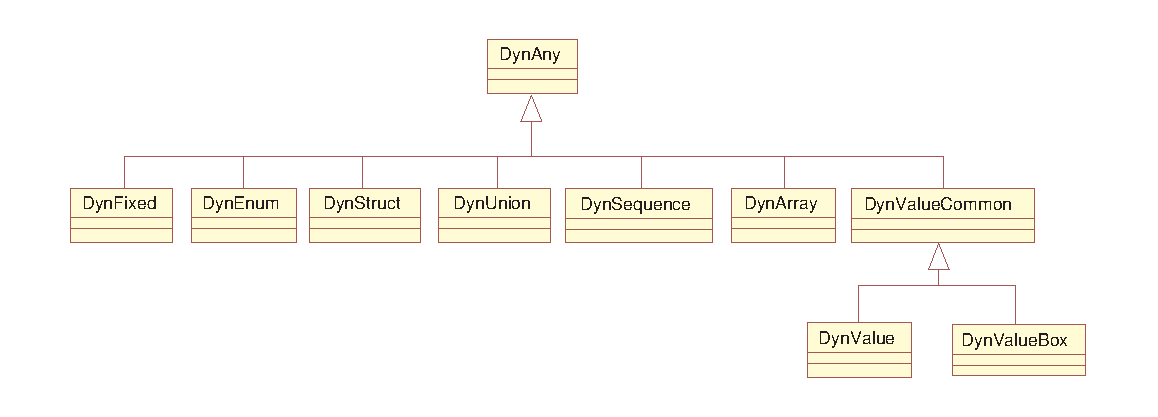
\includegraphics[width=\textwidth]{dynany}
  \end{center}
\caption{DynAny Relationships}
\end{figure}


The DynAny interface is the base interface that represents values of
the basic types.  For each constructed type there is a corresponding
interface that extends the DynAny interface and defines operations
specific to the constructed type.  The table below lists the
interfaces in the DynamicAny module and the types they represent.


\begin{small}
\begin{longtable}{|p{6.3cm}|p{8.6cm}|}
\hline
~ \hfill \textbf {Interface} \hfill ~ & ~ \hfill \textbf {Type} \hfill ~ \endhead
\hline
\verb"DynAny" & \verb"basic types (boolean, long, etc.)" \\
\hline
\verb"DynFixed" & \verb"fixed" \\
\hline
\verb"DynEnum" & \verb"enum" \\
\hline
\verb"DynStruct" & \verb"struct" \\
\hline
\verb"DynUnion" & \verb"union" \\
\hline
\verb"DynSequence" & \verb"sequence" \\
\hline
\verb"DynArray" & \verb"array" \\
\hline
\verb"DynValue*" & \verb"non-boxed valuetype" \\
\hline
\verb"DynValueBox*" & \verb"boxed valuetype" \\
\hline

\end{longtable}
\end{small}

* Not currently implemented by JacORB.

\section{Usage Constraints}

Objects that implement interfaces in the DynamicAny module are
intended to be local to the process that constructs and uses them.
As a result, references to these objects cannot be exported to other
processes or externalized using ORB::object\_to\_string;  an
operation that attempts to do so will throw the MARSHAL system
exception.

\section{Creating a DynAny Object}

The DynAnyFactory interface is used to create a DynAny object.  There
are two operations for creating a DynAny object; these are listed in
the table below.


\begin{small}
\begin{longtable}{|p{6.3cm}|p{8.6cm}|}
\hline
~ \hfill \textbf {Operation} \hfill ~ & ~ \hfill \textbf {Description} \hfill ~ \endhead
\hline
\verb"create_dyn_any" & \verb"Constructs a DynAny object from an Any"
\verb"value" \\
\hline
\verb"create_dyn_any_from_ty"
\verb"pe_code" & \verb"Constructs a DynAny object from a"
\verb"TypeCode" \\
\hline

\end{longtable}
\end{small}

The example below illustrates how to obtain a reference to the
DynAnyFacory object and then use it to construct a DynAny object with
each of the create operations.  Exception handling is omitted for
brevity.

The following line of code imports the classes in the DynamicAny
package.

\begin{small}
\begin{verbatim}
import org.omg.DynamicAny.*;

\end{verbatim}
\end{small}

The following code segment obtains a reference to the DynAnyFacory
object.

\begin{small}
\begin{verbatim}
DynAnyFactory factory = null;
DynAny DynAny = null;
DynAny DynAny2 = null;
org.omg.CORBA.Any any = null;
org.omg.CORBA.TypeCode tc = null;
org.omg.CORBA.Object obj = null;

// obtain a reference to the DynAnyFactory
obj = orb.resolve_initial_references ("DynAnyFactory");

// narrow the reference to the correct type
factory = DynAnyFactoryHelper.narrow (obj);

\end{verbatim}
\end{small}

The following code segment creates a DynAny with each of the create
operations.

\begin{small}
\begin{verbatim}
// create a DynAny object from an Any
any = orb.create_any ();
any.insert_long (1);
DynAny = factory.create_dyn_any (any);

// create a DynAny object from a TypeCode
tc = orb.get_primitive_tc (org.omg.CORBA.TCKind.tk_long);
DynAny2 = factory.create_dyn_any_from_type_code (tc);

\end{verbatim}
\end{small}

If the Any value or TypeCode represents a constructed type then the
DynAny can be narrowed to the appropriate subtype, as illustrated
below.

The following IDL defines a struct type.

\begin{small}
\begin{verbatim}
// example struct type
struct StructType
{
   long field1;
   string field2;
};

\end{verbatim}
\end{small}

The following code segment illustrates the creation of a DynStruct
object that represents a value of type StructType.

\begin{small}
\begin{verbatim}
StructType type = null;
DynStruct dynStruct = null;

// create an Any that contains an object of type StructType
type = new StructType (999, "Hello");
any = orb.create_any ();
StructTypeHelper.insert (any, type);

// construct a DynAny from an Any and narrow it to a DynStruct
dynStruct = (DynStruct) factory.create_dyn_any (any);

\end{verbatim}
\end{small}

\section{Accessing the Value of a DynAny Object}

The DynAny interface defines a set of operations for accessing the
value of a basic type represented by a DynAny object.  The operation
to get a value of basic type $<$type$>$ from a DynAny has the form
get\_$<$type$>$.  The operation to insert a value of basic type
$<$type$>$ into a DynAny has the form insert\_$<$type$>$.  A
TypeMismatch exception is thrown if the type of the operation used to
get/insert a value into a DynAny object does not match the type of
the DynAny.

The operations for accessing the value of a constructed type
represented by a DynAny are defined in the interface specific to the
constructed type.  For example, the DynStruct interface defines the
operation get\_members, which returns a sequence of name/value pairs
representing the members of the struct or exception represented by a
DynStruct object.

\section{Traversing the Value of a DynAny Object}

DynAny objects can be viewed as an ordered collection of component
DynAnys.  For example, in a DynStruct object the ordered collection
of component DynAnys is the members of the struct or exception it
represents.  For DynAny objects representing basic types or
constructed types that do not have components, the collection of
component DynAnys is empty.

All DynAny objects have a current position.  For DynAnys representing
constructed types that have components, the current position is the
index of the component DynAny that would be obtained by a call to the
current\_component operation (described in the table below).  The
component DynAnys of a DynAny object are indexed from 0 to n-1, where
n is the number of components.  For DynAnys representing basic types,
or constructed types that do not have components, the current
position is fixed at the value -1.

The operations for traversing the component DynAnys of a DynAny
object are common to all DynAny subtypes, hence they are defined in
the DynAny base interface.  The table below lists the operations
available for traversing a DynAny object.


\begin{small}
\begin{longtable}{|p{6.3cm}|p{8.6cm}|}
\hline
~ \hfill \textbf {Operation} \hfill ~ & ~ \hfill \textbf {Description} \hfill ~ \endhead
\hline
\verb"seek" & \verb"Sets the current position to the"
\verb"specified index" \\
\hline
\verb"rewind" & \verb"Sets the current position to the first"
\verb"component (index 0)" \\
\hline
\verb"next" & \verb"Advances the current position to the"
\verb"next component" \\
\hline
\verb"component_count" & \verb"Returns the number of components" \\
\hline
\verb"current_component" & \verb"Returns the component at the current"
\verb"position" \\
\hline

\end{longtable}
\end{small}

The following code segment illustrates one way of traversing the
component DynAnys of a DynStruct object.  As the DynStruct is
traversed, the value of each component is obtained and printed.
Exception handling is omitted for brevity.

\begin{small}
\begin{verbatim}
DynAny curComp = null;

// print the value of the first component
curComp = dynStruct.current_component ();
System.out.println ("field1 = " + curComp.get_long ());

// advance to the next component
dynStruct.next ();

// print the value of the second component
curComp = dynStruct.current_component ();
System.out.println ("field2 = " + curComp.get_string ());

\end{verbatim}
\end{small}

The next code segment illustrates another way to perform the same
task.

\begin{small}
\begin{verbatim}
// go back to the first component
dynStruct.rewind ();  // same as calling seek (0)

// print the value of the first component
System.out.println ("field1 = " + dynStruct.get_long ());

// advance to the next component
dynStruct.seek (1);

// print the value of the second component
System.out.println ("field2 = " + dynStruct.get_string ());

\end{verbatim}
\end{small}

As the second code segment illustrates, if the component DynAny
represents a basic type, its value can be extracted (or inserted) by
calling the accessor operation on the parent DynAny directly, rather
than first obtaining the component using the current\_component
operation.

\section{Constructed Types}

This section describes the interfaces in the DynamicAny module that
represent the constructed types supported by JacORB.  Each of these
interfaces extends the DynAny interface.



\subsection{DynFixed}

A DynFixed object represents a fixed value.  Since IDL does not have
a generic type to represent a fixed type, the operations in this
interface use the IDL string type.  The value represented by a
DynFixed object can be accessed (as a string) using the get\_value
and set\_value operations.

A DynFixed object has no components.

\subsection{DynEnum}

A DynEnum object represents a single enumerated value.  The integer
(ordinal) value of the enumerated value can be accessed with the
get\_as\_ulong and set\_as\_ulong operations.  The string (IDL
identifier) value of the enumerated value can be accessed with the
get\_as\_string and set\_as\_string operations.

A DynEnum object has no components.

\subsection{DynStruct}

A DynStruct object represents a struct value or an exception value.
The current\_member\_name and current\_member\_kind operations return
the name and TCKind value of the TypeCode of the member at the
current position of the DynStruct.  The members of the DynStruct can
be accessed with the get\_members and set\_members operations.

The component DynAnys of a DynStruct object are the members of the
struct or exception.  A DynStruct representing an empty exception has
no components.

\subsection{DynUnion}

A DynUnion object represents a union value.  The value of the
discriminator can be accessed using the get\_discriminator and
set\_discriminator operations.

If the discriminator is set to a value that names a member of the
union then that member becomes active.  Otherwise, if the value of
the discriminator does not name a member of the union then there is
no active member.

If there is an active member, the member operation returns its value
as a DynAny object, and the member\_name and member\_kind operations
return its name and the TCKind value of its TypeCode.  These
operations throw an InvalidValue exception if the union has no active
member.

A DynUnion object can have either one or two components.  The first
component is always the discriminator value.  The second component is
the value of the active member, if one exists.

\subsection{DynSequence}

A DynSequence object represents a sequence.  The length of the
sequence can be accessed using the get\_length and set\_length
operations.  The elements of the sequence can be accessed using the
get\_elements and set\_elements operations.

The component DynAnys of a DynSequence object are the elements of the
sequence.

\subsection{DynArray}

A DynArray object represents an array.  The elements of the array can
be accessed using the get\_elements and set\_elements operations.

The component DynAnys of a DynArray object are the elements of the
array.

\section{Converting between Any and DynAny Objects}

The DynAny interface defines operations for converting between Any
objects and DynAny objects.  The from\_any operation initialises the
value of a DynAny with the value of a specified Any.  A TypeMismatch
exception is thrown if the type of the Any does not match the type of
the DynAny.  The to\_any operation creates an Any from a DynAny.

As an example of how these operations might be useful, suppose one
wants to dynamically modify the contents of some constructed type,
such as a struct, which is represented as an Any.  The following
steps will accomplish this task:

\begin{enumerate}
  \item  A DynStruct object is constructed from the TypeCode of the struct using the DynAnyFactory::create\_dyn\_any\_from\_type\_code operation.
  \item  The DynAny::from\_any operation is used to initialise the value of the DynStruct with the value of the Any.
  \item  The contents of the DynStruct can now be traversed and modified.
  \item  A new Any can be created to represent the modified struct using the DynAny::to\_any operation.
\end{enumerate}

\section{Further Examples}

The demo/dynany directory of the JacORB repository contains example
code illustrating the use of DynAny objects.  Further code can be
found in the org.jacorb.test.orb.dynany package of the JacORB-Test
repository.


%%%%%%%%%%%%%%%%%%%%%%%%%%%%%%%%%%%%%%%%%%%%%%%%%%%%%%%%%%%%%%%%%%%%%%%%%%%%%%
\chapter{Objects By Value}
\label{ch:obv}

Until CORBA 2.3, objects could only be passed using reference
semantics: there was no way to specify that object state should be
copied along with an object reference. A further restrictions of the
earlier CORBA version were that all non-object types (structs, unions,
sequences, etc.) were {\em values}, so you could not use, e.g. a
reference to struct to construct a graph of structure values that
contains shared nodes. Finally, there was no inheritance between
structs.

All these shortcomings are addressed the {\em objects-by-value} (OBV)
chapters of the CORBA specification: the addition of stateful
valuetypes supports copy semantics for objects and inheritance for
structs, boxed value types introduce reference semantics for base
types, and abstract interfaces determine whether an argument is sent
by-value or by-reference by the argument's runtime type. The
introduction of OBV into CORBA presented a major shift in the CORBA
philosophy, which had been to strictly avoid any dependence on
implementation details (state, in particular). It also added a
considerable amount of marshaling complexity and interoperability
problems. (As a personal note: Even in CORBA 2.6, the OBV marshalling
sections are still not particularly precise...)

Beginning with the 1.4 beta releases, JacORB added OBV support.
However, the value type support in JacORB is not yet complete: while
the IDL compiler accepts all of the value type IDL syntax, the runtime
system does not support abstract valuetypes, and the marshalling of
truncatable value types does not yet meet all the standard's
requirements (and should thus be called ``beta''). Boxed value types
and simple regular value types (including value type inheritance) work
as prescribed in the standard.

\section{Example}

The remainder of this chapter presents a simple value type example,
which is part of the demo programs in the JacORB distribution. The
demo shows the use of boxed value types and a simple stateful value
type. Here's the IDL definition from {\tt demo/value/server.idl}:

\begin{verbatim}
module demo {
  module value {

     valuetype boxedLong   long;
     valuetype boxedString string;

     valuetype Node {
        public long id;
        public Node next;
     };

     interface ValueServer {
        string receive_long   (in boxedLong p1, in boxedLong p2);
        string receive_string (in boxedString s1, in boxedString s2);
        string receive_list   (in Node node);
     };
  };
};
\end{verbatim}

From the definition of the  boxed valuetype {\tt boxedLong} and
{\tt boxedString}, the IDL generates the following Java class, which
is simply a holder vor the long value. No mapped class is generated
for the boxed string value type.

\begin{verbatim}
package demo.value;

public class boxedLong
    implements org.omg.CORBA.portable.ValueBase
{
    public int value;
    private static String[] _ids = { boxedLongHelper.id() };

    public boxedLong(int initial )
    {
        value = initial;
    }
    public String[] _truncatable_ids()
    {
        return _ids;
    }
}
\end{verbatim}

\subsubsection{Reference Semantics}

The boxed value definitions in IDL above permit uses of non-object
types that are not possible with IDL primitive type. In particular, it
is possible to pass Java {\tt null} references where a value of a
boxed value type is expected. For example, we can call the operation
{\tt receive\_long} and pass one initialized {\tt boxedLong} value and
a null reference, as show in the following snippet from the client
code:

\begin{verbatim}
    ValueServer s = ValueServerHelper.narrow( obj );
    boxedLong boxL = new boxedLong (774);

    System.out.println ("Passing two integers: "
                       + s.receive_long ( boxL , null ));
\end{verbatim}

With a regular {\tt long} parameter, a {\tt null} reference would have
resulted in a {\tt BAD\_PARAM} exception. With boxed valuetypes, this
usage is entirely legal and the result string returned from the {\tt
  ValueServer} object is {\tt ``one or two null values''}.

A second new possibility of the reference semantics that can be
achieved by ``boxing'' primitive IDL types is {\em sharing} of values.
With primitive values, two variables can have copies of the same
value, but they cannot both refer to the same value. This means that
when one of the variables is changed, the other one retains its
orignal value. With shared values that are {\em referenced}, both
variables would always point to the same value.


%%%%%%%%%%%%%%%%%%%%%%%%%%%%%%%%%%%%%%%%%%%%%%%%%%%%%%%%%%%%%%%%%%%%%%%%%%%%%%
\chapter{Interface Repository}
\label{ch:interface_repository}

Run--time  type information  in CORBA  is  managed by  the ORB's  {\it
Interface Repository}  (IR) component.  It allows  to request, inspect
and modify IDL  type information dynamically, e.g., to  find out which
operations an object supports. Some ORBs  may also need the IR to find
out whether  a given object's type  is a subtype of  another, but most
ORBs can do  without the IR by encoding this  kind of type information
in the helper classes generated by the IDL compiler.

In essence,  the IR is  just another remotely accessible  CORBA object
that offers  operations to retrieve  (and in theory also  modify) type
information.

\section{Type Information in the IR}

The  IR  manages  type   information  in  a  hierarchical  containment
structure that  corresponds to the structure of  scoping constructs in
IDL  specifications:   modules  contain  definitions   of  interfaces,
structures, constants  etc. Interfaces in turn  contain definitions of
exceptions, operations, attributes  and constants. Figure \ref{IR-fig}
illustrates this hierarchy.

\begin{figure}[htb]
  \begin{center}
    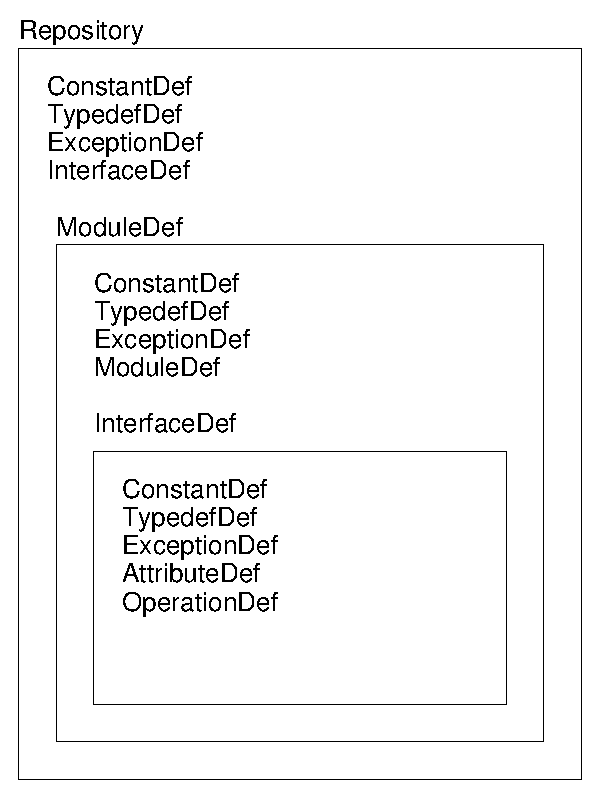
\includegraphics[width=5cm]{IR}
  \end{center}
\caption{Containers in the Interface Repository}
\label{IR-fig}
\end{figure}

The  descriptions  inside  the  IR  can  be  identified  in  different
ways. Every  element of  the repository has  a unique,  qualified name
which  corresponds  to  the  structure  of  name  scopes  in  the  IDL
specification. An interface {\tt  I1} which was declared inside module
{\tt M2} which in turn was  declared inside module {\tt M1} thus has a
qualified name  {\tt M1::M2::I1}. The  IR also provides  another, much
more   flexible   way   of    naming   IDL   constructs   using   {\it
Repository Id}s.  There   are  a   number  of  different   formats  for
RepositoryIds  but  every  Repository  must  be  able  to  handle  the
following format, which is marked  by the prefix {\tt "IDL:"} and also
carries  a  suffix   with  a  version  number,  as   in,  e.g.,  "{\tt
IDL:jacorb/demo/grid:1.0}". The name  component between the colons can
be set freely using the  IDL compiler directives {\tt \#pragma prefix}
and {\tt \#pragma ID}. If no such directive is used, it corresponds to
the qualified name as above.

\section{Repository Design}

When designing the  Interface Repository, our goal was  to exploit the
Java reflection  API's functionality to  avoid having to  implement an
additional data base for  IDL type descriptions. An alternative design
is to use the IR as a back-end to the IDL compiler, but we did not want
to  introduce such  a  dependency and  preferred  to a  have a  rather
``light--weight'' repository  server.  As  it turned out,  this design
was  possible because  the similarities  between the  Java  and CORBA
object models allow  us to derive the required  IDL information at run
time. As  a consequence,  we can  even do without  any IDL  at compile
time.  In addition  to this simplification, the main  advantage of our
approach lies in avoiding  redundant data and possible inconsistencies
between  persistent IDL descriptions  and their  Java representations,
because Java classes have to be generated and stored anyway.

Thus, the  Repository has to  load Java classes, interpret  them using
reflection  and   translate  them   into  the  appropriate   IDL  meta
information. To  this end, the  repository realizes a  reverse mapping
from   Java   to  IDL.   Figure   \ref{IR-Process}  illustrates   this
functionality,  where $f^{-1}$  denotes  the reverse  mapping, or  the
inverse of  the language  mapping.

\begin{figure}[htb]
  \begin{center}
    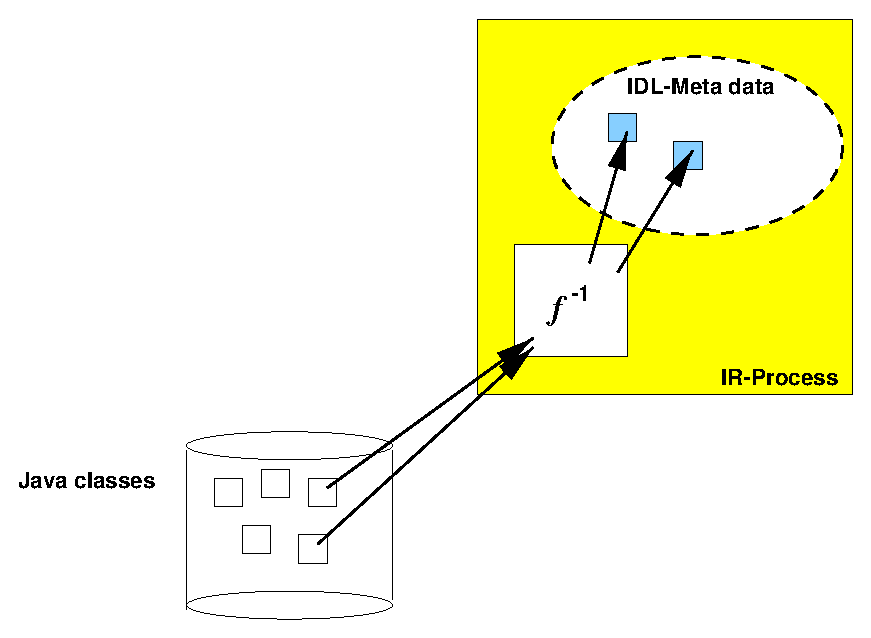
\includegraphics[width=7cm]{IR-Process}
\end{center}
\caption{The JacORB Interface Repository}
\label{IR-Process}
\end{figure}

\section{Using the IR}

For the ORB to be able to contact the IR, the IR server process must
be running. To start it, simply type the {\tt ir} command and provide
the required arguments:

\cmdline{ir /home/brose/classes /home/brose/public\_html/IR\_Ref}

The first  argument is  a path to  a directory containing  {\tt .class}
files and packages. The IR  loads these classes and tries to interpret
them as  IDL compiler--generated classes.  If it  succeeds, it creates
internal representations  of the  adequate IDL constructs.  The second
argument on  the command  line above  is simply the  name of  the file
where the IR stores its object reference for ORB bootstrapping.

To view the contents of the repository, you can use the GUI IRBrowser
tool or the query command. First, let's query the IR for a particular
repository ID. JacORB provides the command {\tt qir} (``query IR'')
for this purpose:

\cmdline{qir IDL:raccoon/test/cyberchair/Paper:1.0}

As result, the IR returns an InterfaceDef object, and {\tt qir} parses
this and prints out:

\begin{verbatim}
     interface Paper
     {
        void read(out string arg_0);
        raccoon::test::cyberchair::Review getReview(in long arg_0);
        raccoon::test::cyberchair::Review submitReview(
            in string arg_0, in long a rg_1);
        void listReviews(out string arg_0);
     };
\end{verbatim}

To start the IRBrowser, simply type

\cmdline{irbrowser}

Figure \ref{fig:IRBrowser} gives a screen shot of the IR browser.

\bigskip
\begin{figure}[htb]
  \begin{center}
    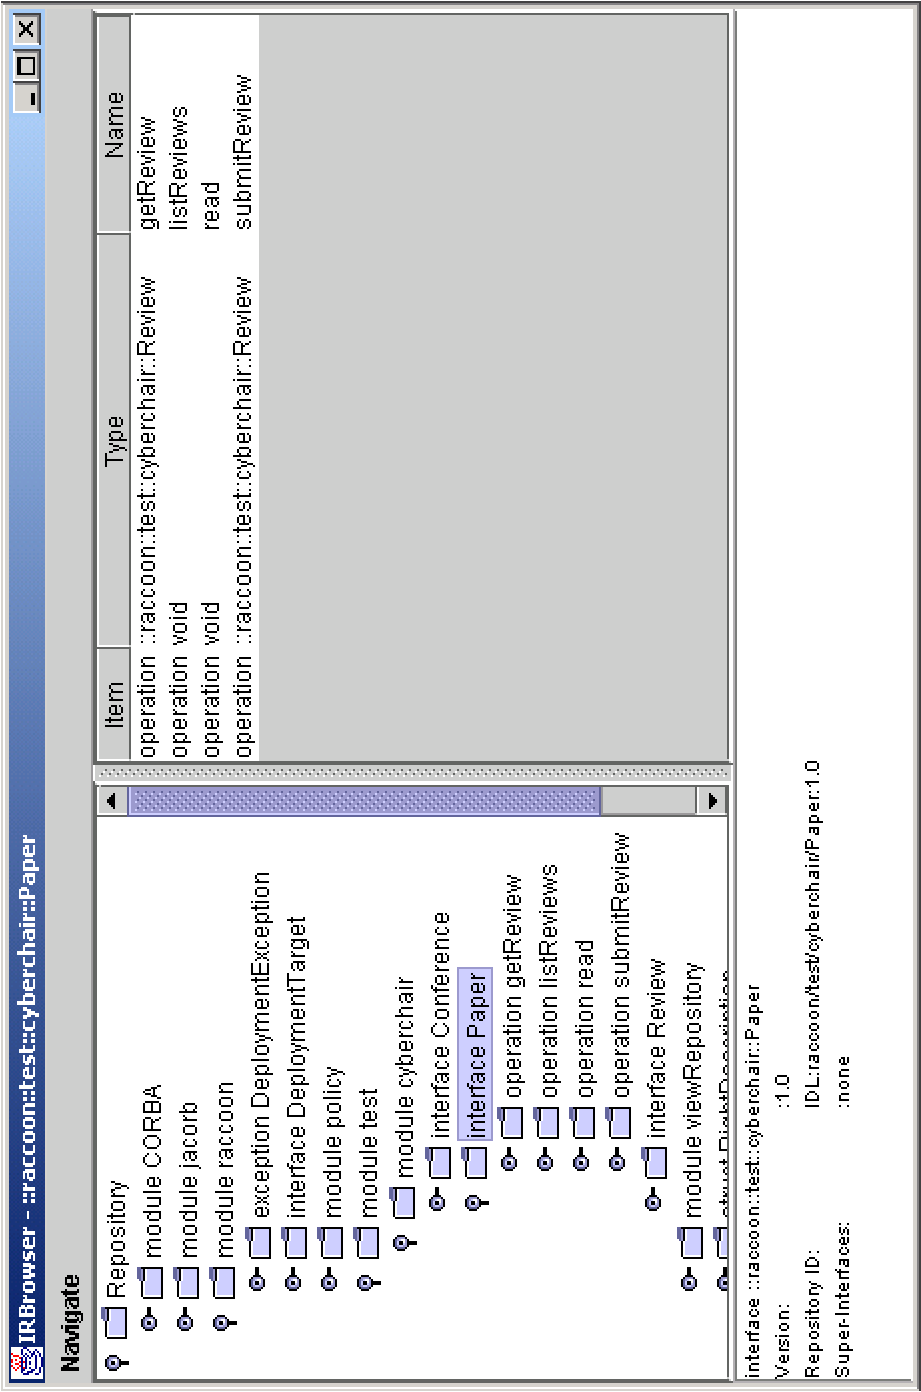
\includegraphics[width=11cm]{IRBrowser}
\end{center}
\caption{IRBrowser Screenshot}
\label{fig:IRBrowser}
\end{figure}

The Java classes generated by  the IDL compiler using the standard OMG
IDL/Java language mapping do not contain enough information to rebuild
all  of the  information contained  in  the original  IDL file.   For
example,  determining whether an  attribute in  an interface  was {\tt
readonly} or  not is not  possible, or telling the  difference between
{\tt  in}  and {\tt  inout}  parameter  passing  modes. Moreover,  IDL
modules are not  explicitly represented in Java, so  telling whether a
directory in  the class  path represents an  IDL module is  not easily
possible. For these  reasons, the JacORB IDL compiler  generates a few
additional  classes that hold  the required  extra information  if the
compiler switch {\tt -ir} is used when compiling IDL files:

\cmdline{idl -ir myIdlFile.idl}

The additional files generated by the compiler are:
\begin{itemize}
\item a {\tt \_XModule.java} class file for any IDL module X
\item a {\tt YIRHelper.java} class file for any interface Y.
\end{itemize}

If no  {\tt .class} files that  are compiled from  these extra classes
are found  in the class path passed  to the IR server  process, the IR
will not  be able  to derive any  representations.  Note that  the IDL
compiler does not make any non--compliant modifications to any of the
standard files that are defined in the Java language mapping --- there
is only additional information.

One more caveat about these  extra classes: The compiler generates the
{\tt  \_XModule.java} class  only  for genuine  modules. Java  package
scopes created by applying the {\tt -d } switch to the IDL compiler do
not  represent   proper  modules  and   thus  do  not   generate  this
class. Thus, the contents of  these directories will not be considered
by the IR.

When an  object's client  calls the {\tt  get\_interface()} operation,
the ORB consults the IR  and returns an {\tt InterfaceDef} object that
describes the object's  interface. Using {\tt InterfaceDef} operations
on  this  description  object,  further  description  objects  can  be
obtained,  such as descriptions  for operations  or attributes  of the
interface under consideration.

The IR  can also be  called like any  other CORBA object  and provides
{\tt lookup()}  or {\tt lookup\_name()} operations to  clients so that
definitions can be searched for, given a qualified name. Moreover, the
complete contents of individual containers (modules or interfaces) can
be listed.

Interface   Repository  meta   objects  provide   further  description
operations. For a given {\tt  InterfaceDef} object, we can inspect the
different  meta   objects  contained   in  this  object   (e.g.,  {\tt
OperationDef} objects). It is  also possible to obtain descriptions in
form of a simple structure  of type {\tt InterfaceDescription} or {\tt
FullInterfaceDescription}. Since structures are  passed by value and a
{\tt   FullInterfaceDescription}    fully   provides   all   contained
descriptions,  no  further  ---possibly  remote  ---  invocations  are
necessary for searching the structure.


%%%%%%%%%%%%%%%%%%%%%%%%%%%%%%%%%%%%%%%%%%%%%%%%%%%%%%%%%%%%%%%%%%%%%%%%%%%%%%
\chapter{The JacORB Appligator}
\label{Ch_applets}

{\em by Sebastian M{\"u}ller and Steve Osselton}

\bigskip

Version 1.4 of JacORB includes a new implementation of the Appligator.
This is a portable interceptor based IIOP proxy.  Using this proxy you
can both run Java Applets with JacORB and use JacORB across firewalls
and the Internet. This new implementation no longer supports HTTP
tunneling.

\section{Appligator Functionality}

The Appligator is a GIOP proxy. When the Appligator is used, instead
of a client calling directly to a server it calls to the Appligator
which then itself calls on to the server. This is all transparent as
far as a client is concerned.  The basic mechanism of operation is as
follows:

\begin{enumerate}
\item A client that wishes to use the Appligator installs a client
  side interceptor.
\item When the client makes a call the interceptor checks to determine
  whether the call should be redirected to an Appligator. If so, then
  the original call target is encoded within a service context and a
  ForwardRequest exception is thrown so that the ORB redirects the
  call to the Appligator.
\item When the Appligator receives a forwarded request it extracts the
  original target from the service context and calls onto the original
  target. The actual proxy implementation within the Appligator is
  invoked via DSI and calls on to the target via DII.
\end{enumerate}

\section{Using The Appligator}

The Appligator can be run as a normal CORBA server via the
'appligator' shell script or batch file. The Appligator is configured
vis both command line arguments and properties stored in the ORB
configuration file 'jacorb.properties'.

\subsection{Starting Appligator}

The Appligator can be invoked as follows:

\verb+$ appligator <port> <filename> [-dynamic]+

This starts the Appligator on the specified port and writes it's IOR
to the specified file.

The '-dynamic' flag is optional and determines whether the object key
used for the Appligator IOR is dynamically (i.e. randomly) selected or
fixed. If a fixed id is used then the configuration property
'jacorb.ProxyServer.ID' is used as the object key value. If this is
not set then this defaults to 'Appligator'. Using a fixed object key
has the advantage that this key is used every time the Appligator
restarts so a remote client would not have to update it's reference to
the Appligator (typically an IOR file).

\subsection{Client Configuration}

Appligator clients need to install the appropriate client side
interceptor class. This can be done by configuring the portable ORB
initializer class 'ProxyClientInitializer' by setting the following
ORB initialization property:

{\noindent\tt\small
  org.omg.PortableInterceptor.ORBInitializerClass.org.jacorb.\\
proxy.ProxyClientInitializer}

\subsection{Appligator Configuration Appligator}

configuration properties are
placed in the 'jacorb.properties' file, all have the common prefix
'jacorb.ProxyServer'. Configuration properties are used either for the
configuration of the Appligator server itself or for the configuration
of Appligator clients.

\subsubsection{Appligator Server Properties}

If the 'jacorb.ProxyServer.Name' property is set and the name service
has been configured and is available then the Appligator will register
itself in the name service using this name.  If the
'jacorb.ProxyServer.ID' property is set and the Appligator has not
been run with the '-dynamic' flag then this property is used as the
object key in the created Appligator IOR.

\subsubsection{Appligator Client Properties}

The 'jacorb.ProxyServer.URL' configuration property is used
by clients to locate the default Appligator. This URL should map to an
IOR file written by an Appligator.  If the
'jacorb.ProxyServer.Network' and 'jacorb.ProxyServer.Netmask'
properties are set these are used to determine the local network
address for a client. If this is set then any calls to objects within
this network will not be redirected to the Appligator. This is useful
when a CORBA server may need to call to an Appligator to access remote
servers but may want to communicate with local servers directly. The
dotted decimal form should be used for both these properties, for
example:

\verb+jacorb.ProxyServer.Netmask=255.255.255.0+

\verb+jacorb.ProxyServer.Network=160.45.110.0+

Clients can be configured to use different Appligators to access
objects in different subnets. To do this configuration properties of
the form 'jacorb.ProxyServer.URL-<network>-<netmask>' can be
used. Here the URL property should map to the Appligator IOR for the
particular subnet identified by <network> and <netmask>. For example:

\verb+jacorb.ProxyServer.URL-160.45.120.0-255.255.255.0=file:/tmp/net1.ior+

\section{Applet Support}

Regular Java programs can connect to every host on the Internet,
applets can only open connections to their applethost (the host they
are downloaded from). This lets Applets only use CORBA servers on
their applethost, if no proxy is used. With JacORB Appligator, access
for your Applets is no longer restricted. Placed on the applethost,
Appligator handles all connections from and to your Applet
transparently.

Due to the transparency of JacORB Appligator you can write your Applet
as if it were a normal CORBA program. The only thing you have to do is
to use a special initialization of the ORB by calling the ORB init
operation that takes an Applet as a parameter:

\verb+ORB orb = ORB.init (applet, properties);+

A normal JacORB program reads a local jacorb.properties file to get
the URL of its name server and other vital settings. An Applet of
course has no local properties file, but a remote one: You have to
place the properties file (which has the same syntax and parameters as
the normal file) in the same directory as your Applet (the file name
has to be: jacorb.properties, without a leading dot).

Similar to the name server, Appligator writes its IOR to a file. Your
Applet has to know the location of this file to retrieve the IOR of
Appligator. You must set the location of the IOR file via the
jacorb.properties file (jacorb.ProxyServer.URL) or with an Applet
parameter in the <APPLET> HTML tag (JacorbProxyServerURL).

\subsection{Summary}

\begin{itemize}
\item Init the ORB with jacorb.orb.init(applet,properties), where applet is
this Applet and properties are java.util.Properties (which can be
null).
\item Put a jacorb.properties file in the directory of the Applet.
\item Specify the location for the Appligator IOR file in the
jacorb.properties (jacorb.ProxyServer.URL) or in an Applet parameter
(JacorbProxyServerURL)
\item Make sure the name server IOR file is
accessible for the Applet (lies on the applethost)
\item Start Appligator on the applethost (web server) with:

\verb+$ appligator <port> <filename>+

Where filename is the location where the Appligator IOR is written and is the location specified in the JacORB properties file or Applet parameter.
\end{itemize}

\subsection{Applet Properties}

As described above there are some ways for the Applet to get its JacORB properties file. The most important property is the URL to the Appligator IOR file. Without this property the Applet will not work. If you use a name server, the URL to the name server IOR must also be specified.

Properties can be set in three ways:
\begin{enumerate}
\item In the ORB.init() call with the java.util.Properties parameter.
\item In the JacORB properties file located in the same directory as
  the Applet
\item The URL to the name server and Appligator IOR file can be set in
  the Applet tag in the HTML file
\end{enumerate}


\subsection{Appligator and Netscape/IE, appletviewer}

Netscape Navigator/Communicator comes with its own (outdated) CORBA
support. You have to delete Netscape's CORBA classes to use JacORB. To
do this you have to delete the file iiop10.jar located in NS
ROOT/java/classes. It's a good idea to store a backup of Netscape's
file in another directory. Note that renaming this jar file in the
original directory does not suffice if you don't also change the .jar
extension because Netscape loads all jar files in this directory. You
then need to install jacorb.jar in this directory.

If Netscape loads wrong classes or throws security exceptions (have a
look at Netscape's Java Console to see this) be sure to check your
CLASSPATH and look for old jar files or ``.''. Remove all JacORB and
VisiBroker classes from your CLASSPATH. We succeeded running JacORB
Applet clients on Netscape  4.72 with the Java 1.3 plugin.

Microsoft's Internet Explorer is stricter than Netscape: Even
downloaded classes are not allowed to listen on a socket. We strongly
advise to use Sun's Java 1.3 plugin with IE also. To trick IE into
using JacORB, you need to copy JacORB classes to
\$WINNT$\backslash$Java$\backslash$TrustLib. You can either copy the
entire jacorb.jar and unpack it in this directory or just copy the
directories jacorb, org,and HTTPClient.

Appligator works well with Sun's appletviewer. You only have to make
the appletviewer replace the Sun's CORBA classes with JacORB's
classes. A typical appletviewer call for JacORB Applets looks like
this (written in one command line):

\verb+$ appletviewer http://www.example.com/CORBA/dii example.html+

There is a shell script called ''jacapplet'' in JacORB's bin
directory, which calls the appletviewer with the appropriate options
(you have to edit it to match your local JDK path).

If you use the Appligator with other browsers or if you know a way to
load the JacORB classes without removing and copying jars please let
us know.

\subsection{Examples}

There are some example applets in the demo directory
(jacorb/demo/applet). They are based on the normal examples. The
examples include a HTML file which calls the Applet. To run the
example start the name server first. Start Appligator on your web
server and than the normal example server corresponding to the Applet
example on any computer in any order. Then you can call the example
Applet with the JDK appletviewer or Netscape.

Be sure to have a jacorb.properties file and the jacorb.jar in place.

\section{Firewall Support}

Typically firewalls do two things: filter traffic by port, and filter
traffic by protocol. The JacORB Appligator can be used to deal with
port restrictions.

The Appligator was written to avoid the sandbox restrictions for Java
applets. Unsigned applets can only have connections to the host they
are loaded from, which makes them useless in most distributed CORBA
scenarios. The Appligator is a GIOP proxy, which enables applets to
connect to every CORBA server by redirecting the traffic from the
Applet to the CORBA server to the proxy. The Appligator also works the
other way round: Every connection the Applet is redirected to the
Appligator.

Even without applets the Appligator can be used as a GIOP proxy on a
firewall. The Appligator is a CORBA object itself and is explicitly
started on a given port using a command line argument <port>. All
incoming traffic to the Appligator will go to port <port>. If you
configure your CORBA object behind the firewall to be aware of the
Appligator all traffic from and to this objects will go through the
Appligator.

To make your port filtering firewall working with CORBA and GIOP
messages you must ask your system administrator to assign a port for
GIOP messages on the firewall. Start the Appligator on this port.

Now all CORBA servers (which are aware of the Appligator) in your
enclave can be contacted over the Appligator. If your CORBA client
wants to contact a server in the Internet outside the firewall the
connection will go over the Appligator. Callbacks from the Internet to
your client do not work with Netscape.

Finally you have to specify the location on the Appligator. This is
done the same way as JacORB determines to location of the name server:
When the Appligator starts the IOR of the Appligator is written to a
file which is put to the location you specified as command
parameter. This file must be accessible to all clients that want to
use the Appligator. You can use a shared file system to access this
file or put it on a web server etc. The location of the file in which
the IOR of the Appligator is stored must be set in the
jacorb.properties file. Use the ''jacorb.ProxyServer.URL'' property
for this.

\subsection{Summary}

\begin{itemize}
\item Use the Appligator as a GIOP proxy on a firewall if your
  firewall is configured to block all traffic but traffic on some
  special ports.
\item Ask your system administrator to assign a special port for GIOP
  on your firewall and start the Appligator on this port on the
  firewall: for example:
\verb+$ appligator 7777 app.ior+
\item All CORBA objects that should be reachable from outside the firewall or need to contact a CORBA object outside the firewall must use the Appligator as a proxy. Configure the client side ORB initializer for those applications
\item Set the location of the Appligator in the jacorb.properties file
  of your clients (jacorb.ProxyServer.URL)
\end{itemize}

\subsection{NAT Firewalls}

Most commercial firewalls support Network Address Translation (NAT).
Here the address of an internal server is not made directly visible to
the external Internet, but transformed into another configured address
(typically that of the firewall).

The problem here is that the IOR written by an Appligator will contain
it's internal address. If a remote client wishes to access this
Appligator via a NAT firewall then it cannot use this IOR direct as it
will not contain a routeable address. To support this the Appligator
IOR used by a remote client must be patched to contain the NAT address
of the firewall. A new utility 'fixior' has been provided to do
this. This can be run as follows:

\verb+$ fixior <host> <port> <ior_file>+

\subsection{Security Considerations}

When allowing Appligator traffic through a fixed port in a firewall
the Appligator can in effect allow access to any internal CORBA
server. As the real service target is contained within a service
context a knowledgeable user could attempt to exploit this to access
an unauthorized service. To do this a hacker would have to know the
object key used for the Appligator and a CORBA reference to an
internal service. For this reason if fixed Appligator keys are used it
is recommended that the default value is not used. A much better
solution is to tunnel the Appligator communication through a secure
channel such as afforded by a Secure Shell (SSH) or a Virtual Private
Network (VPN).

\subsection{Use of SSH}

Rather than configure a firewall to allow direct access to an
Appligator a better solution is to enable SSH and use SSH as a secure
tunnel to the Appligator. To do this you first need to patch the
Appligator IOR file used by the client so that this refers to a local
port on the local host:
\verb+$ fixior 127.0.0.1 11111 app.ior+

SSH can then be used to create a secure tunnel between this port and
the remote port on the server machine used by the Appligator. If the
Appligator was running on remote machine 'server' on port 22222 this
could be done as follows:

\verb+$ ssh -T -L 11111:server:22222 server+

If you have a scenario where the server needs to callback to a client
and dual Appligators are deployed on either side of a firewall then
SSH can be used to create a tunnel for each Appligator as follows:

\verb+$ ssh -T -L 11111:server:22222 -R 33333:client:44444 server+

Here SSH has created a local tunnel between port 11111 on 'client' and
port 22222 on 'server' and a remote tunnel between port 33333 on
'server' and port 44444 on 'client'. The 'server' Appligator would be
running on port 22222 and the 'client' Appligator on port 44444. The
Appligator IOR used by 'client' to access the 'server' Appligator
would be patched to have endpoint 127.0.0.1:11111 and the Appligator
IOR used by 'server' to access the 'client' Appligator would be
patched to have endpoint 127.0.0.1:33333.



%%%%%%%%%%%%%%%%%%%%%%%%%%%%%%%%%%%%%%%%%%%%%%%%%%%%%%%%%%%%%%%%%%%%%%%%%%%%%%

\chapter{IIOP over SSL}

\label{SSL}

Using  SSL to authenticate  clients and  to protect  the communication
between client and target requires no changes in your source code. The
only  notable  effect  is  that  SSL/TLS type  sockets  are  used  for
transport  connections  instead of  plain  TCP  sockets  --- and  that
connection setup takes a bit longer.

The only  prerequisites are that you rebuild  JacORB with cryptography
support. You  also need  to set up  a key  store file that  holds your
cryptographic   keys,  and  to   configure  SSL   by  setting   a  few
properties. All of this is described in this chapter.

\section{Re--Building JacORB's security libraries}

In the  standard distribution, the  JacORB security libraries  are not
enabled.   To do  so, you  simply need  to recompile  JacORB  with the
required SSL libraries  in your CLASSPATH.  If these libraries
are not found, JacORB will be rebuilt without SSL support.

To  successfully rebuild  JacORB with  SSL support,  the  following is
required:

\begin{itemize}
        \item when using IAIKs libraries:
              \begin{itemize}
                \item IAIK-JCE 2.591 or later, the security provider classes
                downloadable from \\ \href{http://jcewww.iaik.tu-graz.ac.at}{http://jcewww.iaik.tu-graz.ac.at},
              \item iSaSiLk 3.0 or later, the SSL implementation from the same
                source.
              \end{itemize}

        \item when using Suns libraries:
              \begin{itemize}
              \item JDK 1.4 or jsse1.0.2 available from the Developer
                Connection (for jsse1.0.2, please see the {\tt README.jsse\_1\_0\_2} in
                {\tt src/org/jacorb/security/ssl/sun\_jsse} on how to compile).
              \item For key management, you also need additional packages like
                OpenSSL. These are not necessary for JacORB to work.
              \end{itemize}
\end{itemize}

Install the desired packages and read the documentation carefully. After
successfull installation, build JacORB anew by typing {\tt ant} in your JacORB
installation directory.


\section{IAIK specific setup}
This section covers topics that are specific to IAIKs libraries.

\subsection{Setting up an IAIK key store}

SSL  relies   on  public  key  certificates  in   the  standard  X.509
format. These  certificates are presented in  the authentication phase
of the  SSL handshake and used  to compute and  exchange session keys.
This section explains how to create and store these certificates.

The Java 2  security API provides interfaces that  access a persistent
data structure  called {\em  KeyStore}. A key  store is simply  a file
that contains  public key  certificates and the  corresponding private
keys. It also  contains other certificates that can  be used to verify
public key  certificates.  All  cryptographic data is  protected using
passwords and accessed using names called {\em aliases}.

JacORB provides a  GUI tool to create and  manipulate key store files,
the  KeyStoreManager. It  can generate  key pairs,  sign  public keys,
import  or   export  certificates,  and   define  trusted  certificate
authorities. To start the KeyStoreManager, simply type {\tt ks} on the
command  line. The GUI  lets you  select and  open existing  key store
files, or create new ones.

Starting with an  empty key store, you first need to  create a new key
store and then  a key pair and certificate. Select  {\tt New} from the
{\tt File}  menu to create  a key store,  and then {\tt New}  from the
{\tt Keys} menu.   You will then be asked to provide  a new alias name
for your  new key entry. You also  need to choose a  password. You can
leave  the  algorithm  and  key  length fields  in  the  combobox  menu
unchanged.

\bigskip
\begin{center}
  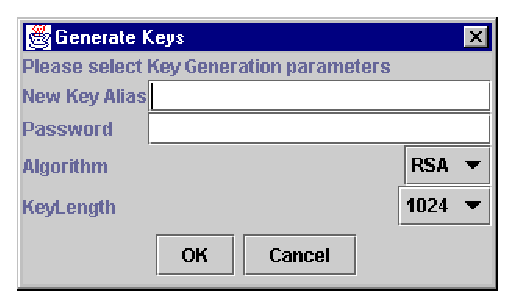
\includegraphics[width=7cm]{Generate}
\end{center}

You  now  have a  public  key certificate  that  you  can present  for
authentication, claiming  identity with the  alias name that  has been
embedded  in the  certificate.   Since anybody  could  present such  a
certificate,  receivers  require  that  the certificate  be  digitally
signed by someone  they trust, a {\em Certificate  Authority} (CA). By
signing  the certificate,  a CA  supports  the identity  claim of  the
certificate  subject. Whose  signature is  accepted as  trustworthy is
just a matter  of configuration, but normally proper  CAs are expected
to only sign certificates that  they have carefully scrutinized --- or
even created themselves.

\bigskip
\centerline{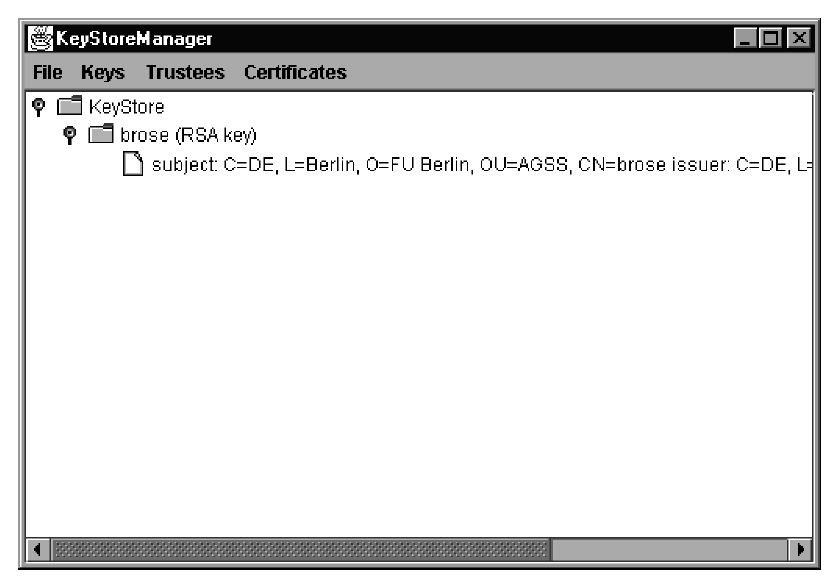
\includegraphics[width=11cm]{Keystore}}

For   convenience  you   can  act   as  a   CA  yourself,   using  the
KeyStoreManager GUI  to import certificates  and then sign  and export
them  again.   The  originating  key  store can  then  re--import  the
certificate that now bears the  digital signature of someone acting as
a CA. The key store has a  standard key chain format that must be used
to store public key certificates. The  first entry in the key chain is
your own public  key certificate as generated by the  key store. It is
automatically signed with its own  private key. Second in the chain is
the public key certificate that is signed by the CA. The last entry in
a key  chain must hold the  CA's public key  certificate, signed using
its private key. Trust in the CA key is ``axiomatic''.

\bigskip
\centerline{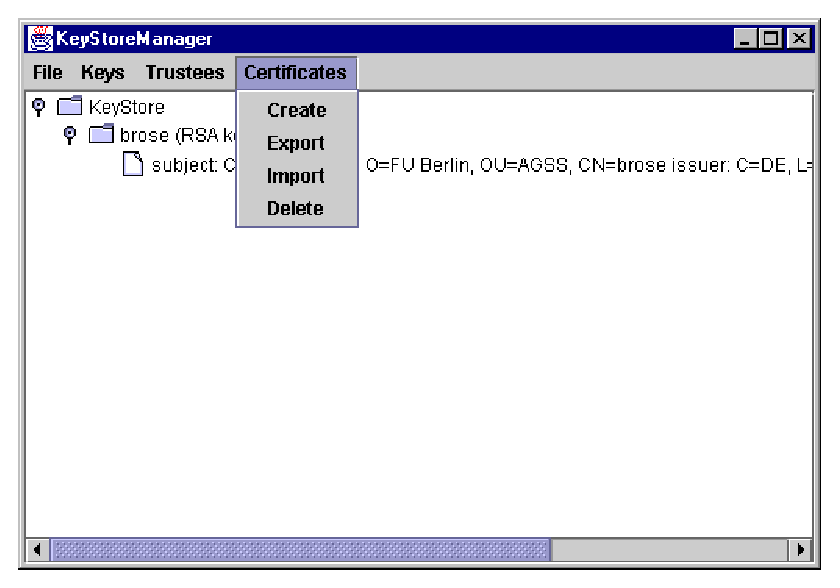
\includegraphics[width=11cm]{KSMenu}}

You can  check the validity of a  key chain by selecting  an alias and
then choosing {\tt Verify Chain}  from the {\tt Keys} menu. Unless the
key  chain  has  the proper  format  {\em  and}  the CA's  public  key
certificate is also declared  as trusted using the {\tt Trustees--add}
menu, the  verification will fail.  Only of  the verification succeeds
will you be able to use a public key certificate in the SSL connection
setup. More documentation on key stores  can be found in the Java tool
documentation for the {\tt keytool}  command. If you care for ``real''
security,  be advised  that setting  up  and managing  (or finding)  a
properly administered CA is essential for the overall security of your
system.

Finally,  note that  key  stores  are normally  used  only for  client
authentication in JacORB.   Servers may, but need not,  have their own
keys and  passwords because server authentication is  optional and not
mandatory like  client authentication. Technically,  this is achieved
by  exchanging the  client  and server  roles  at SSL  setup. This  is
entirely  transparent to  applications, of  course, but  might prevent
interoperation  with other ORBs  over SSL  if their  SSL setup  is not
prepared to handle this role change.

\subsection{Step--By--Step certificate creation}
In  order to  generate  a  simple public  key  infrastructure you  can
perform the following steps:
\begin{enumerate}
\item Create new keystores (File/new) and keypairs (Keys/new) for the CA
and for the user.
\item  Open the  user keystore (File/open),  select the  key  entry and
export the self-signed certificate (Certificates/Export).
\item  Open  the  CA  keystore  and  add the  user  certificate  as  a
Trustee (Trustees/add\dots).
\item Select the  trusted user certificate and create  a signed public
key certificate (Certificates/Create). Leave the role name field empty,
enter the  CAs private  key password and  save the new  certificate by
clicking OK.
\item Export the  CAs self-signed certificate to a  file (as explained
above).    Delete    the    trusted    certificate   from    the    CA
keystore (Trustees/Delete).
\item Open the  user keystore again. Select the  key entry, the import
the CA-signed  user cert (Certificates/Import), and  the self-signed CA
cert.
\item Add  the self-signed CA cert  as a trustee. This  is only needed
for verifying the chain, therefor the keystore can be deployed without
it.  Please  note  that  a  failed  verification  might  result  in  a
SignatureException.
\end{enumerate}

\section{Configuring SSL properties}

When the ORB is initialized by the application, a couple of properties
are read from files and the  command line. To turn on SSL support, you have to
set the following property to ``on'':

\begin{verbatim}
        jacorb.security.support_ssl=on
\end{verbatim}

This will just load the SSL classes on startup. The configuration of the
various aspects of SSL is done via additional properties.

As explained  in the previous  section, cryptographic data  (key pairs
and  certificates) is  stored in  a  keystore  file. To configure the
file name of the keystore file, you need to define the following
property:

\begin{verbatim}
        jacorb.security.keystore=AKeystoreFileName
\end{verbatim}

The keystore file name can either be an absolute path or relative to
the home directory. Keystores are searched in this order, and the
first one found is taken. If this property is not set, the user will be
prompted to enter a keystore location on ORB startup.

To avoid  typing in  lots of  aliases and passwords  (one for  the key
store, and  one for each entry  that is used), you  can define default
aliases and passwords like this:

\begin{verbatim}
# the name of the default key alias to look up in the keystore
jacorb.security.default_user=brose
jacorb.security.default_password=jacorb
\end{verbatim}


These SSL settings can be further refined using security options as in
the following property definitions:

\begin{verbatim}
        jacorb.security.ssl.client.supported_options=0
        jacorb.security.ssl.client.required_options=0

        jacorb.security.ssl.server.supported_options=0
        jacorb.security.ssl.server.required_options=0
\end{verbatim}

The  value  of  these security  options  is  a  bit  mask coded  as  a
hexadecimal integer. The meanings of the individual bits is defined in
the CORBA Security Service  Specification and reproduced here from the
{\tt Security.idl} file:

\begin{verbatim}
        typedef unsigned short   AssociationOptions;

        const AssociationOptions NoProtection = 1;
        const AssociationOptions Integrity = 2;
        const AssociationOptions Confidentiality = 4;
        const AssociationOptions DetectReplay = 8;
        const AssociationOptions DetectMisordering = 16;
        const AssociationOptions EstablishTrustInTarget = 32;
        const AssociationOptions EstablishTrustInClient = 64;
        const AssociationOptions NoDelegation = 128;
        const AssociationOptions SimpleDelegation = 256;
        const AssociationOptions CompositeDelegation = 512;
\end{verbatim}

% With the current SSL integration in JacORB, the only valid settings
% are EstablishTrustInTarget and/or EstablishTrustInClient, i.e.  hex
% values 20, 40 or 60. NoProtection is not possible when SSL is used. If
% you don't want protection, switch SSL support off. The following
% sections go into some more detail about what specific property values
% mean.

\subsection{Client side configuration}

\begin{verbatim}
   jacorb.security.ssl.client.supported_options=20 //EstablishTrustInTarget
\end{verbatim}
This value indicates that the client can use SSL. Actually, this is default
SSL behaviour and must always be supported by the client.

\begin{verbatim}
   jacorb.security.ssl.client.supported_options=40 //EstablishTrustInClient
\end{verbatim}
This makes the client load it's own key/certificate from it's
keystore, because it must be prepared to authenticate to the server.

\begin{verbatim}
   jacorb.security.ssl.client.required_options=20 //EstablishTrustInTarget
\end{verbatim}
This enforces SSL to be used.

\begin{verbatim}
   jacorb.security.ssl.client.required_options=40 //EstablishTrustInClient
\end{verbatim}
This enforces SSL to be used. Actually, this is no meaningfuly value, since in
SSL, the client can't force it's own authentication to the server.


\subsection{Server side configuration}

\begin{verbatim}
   jacorb.security.ssl.server.supported_options=1 //NoProtection
\end{verbatim}
This tells the clients that the server also supports unprotected
connections. If NoProtection is set, no required options should be set as
well, because they override this value.

\begin{verbatim}
   jacorb.security.ssl.server.supported_options=20 //EstablishTrustInTarget
\end{verbatim}
This value indicates that the server supports SSL. Actually, this is default
SSL behaviour and must always be supported by the server. This also makes the
server load it's key/certificate from the keystore.

\begin{verbatim}
   jacorb.security.ssl.server.supported_options=40 //EstablishTrustInClient
\end{verbatim}
This value is ignored, because authenticating the client is either
required, or not done at all (the client can't force its own
authentication).

\begin{verbatim}
   jacorb.security.ssl.server.required_options=20 //EstablishTrustInTarget
\end{verbatim}
This enforces SSL to be used.

\begin{verbatim}
   jacorb.security.ssl.server.required_options=40 //EstablishTrustInClient
\end{verbatim}
This enforces SSL to be used, and will request the client to authenticate. It
also will load trusted certificates for the authentication process.

%%%%%%%%%%%%%%%%%%%%%%%%%%%%%%%%%%%%%%%%%%%%%%%%%%%%%%%%%%%%%%%%%%%%%%%%%%%%%%

\chapter{BiDirectional GIOP}

BiDirectional GIOP has its main use in configurations involving callbacks with
applets or firewalls where it sometimes isn't possible to open a direct
connection to the desired target. As a small example, imagine that you want to
monitor the activities of a server via an applet. This would normally be done
via a callback object that the applet registers at the server, so the applet
doesn't have to poll the server for events. To accomplish this without
BiDirectional GIOP, the server would have to open a new connection to the
client which will not work because applets usually arent allowed to act as
servers, i.e. open ServerSockets. At this point BiDirectional GIOP can help
because it allows to reuse the connection the applet opened to the server for
GIOP requests from the server to the applet (which isn't allowed in
``standard'' GIOP).

\section{Setting up Bidirectional GIOP}

Setting up BiDirectional GIOP consists of two steps:
\begin{enumerate}
\item Setting an ORBInitializer property and  creating the BiDir policy
\item Adding this policy to the servant's POA.
\end{enumerate}

\subsection{Setting the ORBInitializer property}

The first thing that is necessary for BiDirectional GIOP to be available is
the presence of the following property, which can be added by the usual ways
(see section \ref{configuration}):

\begin{verbatim}
   org.omg.PortableInterceptor.ORBInitializerClass.bidir_init=
       org.jacorb.orb.connection.BiDirConnectionInitializer
\end{verbatim}

If this property is present on ORB startup, the corresponding policy factory
and interceptors will be loaded.


\subsection{Creating the BiDir Policy}
Creating the necessary BiDir Policy is done via a policy factory hidden in the
ORB.

\begin{verbatim}
import org.omg.BiDirPolicy.*;
import org.omg.CORBA.*;

[...]

Any any = orb.create_any();
BidirectionalPolicyValueHelper.insert( any, BOTH.value );

Policy p  = orb.create_policy( BIDIRECTIONAL_POLICY_TYPE.value,
                               any );
\end{verbatim}

The value of the new policy is passed to the factory inside of an any. The ORB
is the told to create a policy of the specified type with the specified
value. The newly created policy is then used to create a user POA. Please note
that if {\em any} POA of has this policy set, {\em all} connections will be
enabled for BiDirectional GIOP, that is even those targeted at object of POAs
that don't have this policy set. For the full source code, please have a look
at the bidir demo in the {\tt demo} directory.


\section{Verifying that BiDirectional GIOP is used}
From inside of your application, it is impossible to tell whether requests
arrived over a unidirectional or BiDirectional connection. Therefore, to check
if connections are used in both directions, you can either use a network
monitoring tool or take a look at JacORBs output to tell you if your server
created a new connection to the client, or if the existing one is being
reused.

If the debug level is set to 2 or larger, the following output on the server
side will tell you that a connection is being reused:

\begin{verbatim}
[ ConnectionManager: found conn to target <my IP>:<my port> ]
\end{verbatim}

If, on the other hand, the connection is not being reused, the client will
show the following output:
\begin{verbatim}
[ Opened new server-side TCP/IP transport to <my host>:<my port> ]
\end{verbatim}


\section{TAO interoperability}
There is one problem that may prevent TAO and JacORB to interoperate using
BiDirectional GIOP: If JacORB uses IP addresses as host names (JacORBs
default) and TAO uses DNS names as host names (TAOs default), connections
from JacORB clients to TAO servers will not be reused. If, on the other hand,
both use the same ``format'' for host addresses, interoperability will be
successful. There are two ways to solve this problem:
\begin{enumerate}
\item Use {\tt ``-ORBdotteddecimaladdresses 1''} as an command line argument
  to the TAO server.
\item Recompile JacORB with DNS support (See the INSTALL file for more
  information).
\end{enumerate}


%%%%%%%%%%%%%%%%%%%%%%%%%%%%%%%%%%%%%%%%%%%%%%%%%%%%%%%%%%%%%%%%%%%%%%%%%%%%%%

\chapter{Portable Interceptors}

Since revision 1.1 JacORB provides support for Portable Interceptors These
interceptors are compliant to the standard CORBA specification.  Therefore we
don't provide any documentation on how to program interceptors but supply a
few (hopefully helpful) hints and tips on JacORB specific solutions.

The first  step to have an  interceptor integrated into the  ORB is to
register an {\em  ORBInitializer}. This is done by  setting a property
the following way:
\begin{verbatim}org.omg.PortableInterceptor.ORBInitializerClass.<any_suffix>=
   <orb initializer classname>
\end{verbatim}

For compatibility reasons with the spec, the properties format may also be
like this:

\begin{verbatim}org.omg.PortableInterceptor.ORBInitializerClass.<orb initializer classname>
\end{verbatim}

The suffix  is just to distinguish between  different initializers and
doesn't have to  have any meaningful value. The  value of the property
however has to be the fully qualified classname of the initializer. If
the  verbosity  is  set  to  $\geq  2$  JacORB  will  display  a  {\tt
ClassNotFoundException} in  case the initializers class is  not in the
class path.

An example line might look like:
\begin{verbatim}org.omg.PortableInterceptor.ORBInitializerClass.my_init=
   test.MyInterceptorInitializer
\end{verbatim}

Unfortunately the  interfaces of  the specification don't  provide any
access to  the ORB.  If  you need  access to the  ORB from out  of the
initializer  you  can  cast  the  {\tt  ORBInitInfo}  object  to  {\tt
jacorb. orb.portableInterceptor.ORBInitInfoImpl}   and   call  {\tt
getORB()}  to  get  a  reference  to the  ORB  that  instantiated  the
initializer.

When working with service contexts please make sure that you don't use {\tt
  0x4A414301} as an id because a service context with that id is used
internally.  Otherwise you will end up with either your data not transfered or
unexpected internal exceptions.


%%%%%%%%%%%%%%%%%%%%%%%%%%%%%%%%%%%%%%%%%%%%%%%%%%%%%%%%%%%%%%%%%%%%%%%%%%%%%%

\chapter{Asynchronous Method Invocation}

JacORB allows you to invoke objects asynchronously, as defined in the
\emph{Messaging} chapter of the CORBA specification (chapter 22 in
CORBA 3.0).  Only the callback model is implemented at this time;
there is no support for polling yet.

Asynchronous Method Invocation (AMI) means that when you invoke a
method on an object, control returns to the caller immediately; it
does not block until the reply has been received from the remote
object.  The results of the invocation are delivered later, as soon as
they are received by the client ORB.  Asynchronous Invocation is
entirely a client-side feature.  The server is never aware whether it
is invoked synchronously or asynchronously.

In the callback model, replies are delivered to a special
\emph{ReplyHandler} object that is registered at the client side when
the asynchronous invocation is started.  Here is a brief example for
this (see the \emph{Messaging} specification for further details).
Suppose you have a Server object, defined in a file server.idl.

\begin{verbatim}  interface Server
  {
      long operation (in long p1, inout long p2);
  };
\end{verbatim}

The first step is to compile this IDL definition with the
``ami\_callback'' compiler switch:

\begin{verbatim}  idl -ami_callback server.idl\end{verbatim}

This lets the compiler generate an additional ReplyHandler class,
named AMI\_ServerHandler.  For each operation of the Server interface,
this class has an operation with the same name that receives the
return value and out parameters of the original operation.  There is
an additional method named operation\_excep that is called if the
invocation raises an exception.  If it were defined in IDL, the
ReplyHandler class for the above Server would look like this:

\begin{verbatim}  interface AMI_ServerHandler : Messaging::ReplyHandler
  {
     void operation (in long ami_return_val, in long p2);
     void operation_excep (in Messaging::ExceptionHolder excep_holder);
  };
\end{verbatim}

To implement this interface, extend the corresponding POA class (or
use the tie approach), as with any CORBA object:

\begin{verbatim}  public class AMI_ServerHandlerImpl extends AMI_ServerHandlerPOA
  {
       public void operation (int ami_return_val, int p2)
       {
           System.out.println ("operation reply received");
       }

       public void operation_excep 
                (org.omg.Messaging.ExceptionHolder excep_holder)
       {
           System.out.println ("received an exception");
       }

  }
\end{verbatim}

For each method $m$ of the original Server interface, the IDL compiler
generates a special method sendc\_$m$ into the stub class if the
``ami\_callback'' switch is on.  The parameters of this method are (1)
a reference to a ReplyHandler object, and (2) all \emph{in} or
\emph{inout} parameters of the original operation, with their mode
changed to \emph{in} (\emph{out} parameters are omitted from this
operation).  The sendc operation does not have a return value.

To actually make an asynchronous invocation, an instance of the
ReplyHandler needs to be created, registered with the ORB, and passed
to the sendc method.  The code for this might look as follows:

\begin{verbatim}  ORB    orb = ...
  Server s   = ...

  // create handler and obtain a CORBA reference to it
  AMI_ServerHandler h = new AMI_ServerHandlerImpl()._this (orb);

  // invoke sendc
  ((_ServerStub)s).sendc_operation (h, 4, 5);
\end{verbatim}

Note that the sendc operation is only defined in the stub, and
therefore the cast is necessary to invoke it.  There is not yet any
consensus in the OMG whether the sendc operation should also be
declared in any of the Java interfaces that make up the Server type.
Thus, the fact that you need to make a cast to the stub class
may change in a future version of JacORB.

If you want to try asynchronous invocations with code such as above,
make sure that your client process does something else or at least
waits after the invocation has been made, otherwise it will likely
exit before the reply can be delivered to the handler.

The \emph{Messaging} specification also defines a number of CORBA
policies that allow you to control the timing of asynchronous
invocations.  Since these policies are applicable to both synchronous
and asynchronous invocations, we describe them in a separate section
(see chapter \ref{qos}).

%%%%%%%%%%%%%%%%%%%%%%%%%%%%%%%%%%%%%%%%%%%%%%%%%%%%%%%%%%%%%%%%%%%%%%%%%%%%%%

\chapter{\label{qos}Quality of Service}

JacORB implements a subset of the QoS policies defined in chapter
22.2 of the CORBA 3.0 specification.  In the following, we describe
each of the policies we have currently implemented, along with notes
on particular JacORB issues concerning each policy.  Policies not
listed in the following are not yet implemented.

As of yet, all the policies in this chapter are \emph{client-side
override policies}.  That means that you must specify them for
individual objects, always using the same mechanism:

\begin{description}
\item[Step 1.] Get an Any from the ORB and put the value for the
           policy into it.
\item[Step 2.] Get a Policy object from the ORB which encapsulates the
           desired value (the Any value from the previous step).
\item[Step 3.] Apply the policy to a particular object using
           \emph{\_set\_policy\_override()}.
\end{description}

Here is the code for this, using the \emph{SyncScopePolicy}
(described in the following section) as an example:

\begin{verbatim}
SomeCorbaType     server = ...
org.omg.CORBA.ORB orb    = ...
org.omg.CORBA.Any a      = orb.create_any();
a.insert_short (SYNC_WITH_SERVER.value); // policy value
try
{
    Policy p =
        orb.create_policy(SYNC_SCOPE_POLICY_TYPE.value, a);
    server._set_policy_override (new Policy[]{ p }, 
                                 SetOverrideType.ADD_OVERRIDE);   
}
catch (PolicyError e)
{
    throw new RuntimeException ("policy error: " + e);
}        
\end{verbatim}

Because this is somewhat cumbersome to write, JacORB allows you to
simplify it by creating the Policy object directly via its
constructor:

\newpage

\begin{verbatim}
SomeCorbaType server  = ...

Policy p = new org.jacorb.orb.policies.SyncScopePolicy
                                  (SYNC_WITH_TARGET.value);
server._set_policy_override (new Policy[]{ p },
                             SetOverrideType.ADD_OVERRIDE);
\end{verbatim}

See the package org.jacorb.orb.policies to find out which
constructors are defined for the individual policy types.

\section{Sync Scope}

The \emph{SyncScopePolicy} specifies at which point a oneway
invocation returns to the caller.  (The policy is ignored for
non-oneway invocations.)  There are four possible
values:

\begin{description}
\item[SYNC\_NONE] The invocation returns immediately.
\item[SYNC\_WITH\_TRANSPORT] The invocation returns after the request
  has been passed to the transport layer.
\item[SYNC\_WITH\_SERVER] The server sends an
  acknowledgement back to the client when it has received the
  request, but \emph{before} actually invoking the target.  The
  client-side call blocks until this acknowledgement has been
  received.
\item[SYNC\_WITH\_TARGET] An ordinary reply is sent back by the
  server, \emph{after} the target invocation has completed.  The
  client-side call blocks until this reply has been received.
\end{description}

The default mechanism in JacORB is \emph{SYNC\_WITH\_TRANSPORT},
since the call to the socket layer is a synchronous one.  In order to
implement \emph{SYNC\_NONE}, an additional thread is created on the
fly which in turn calls the socket layer, while the client-side
invocation returns after this thread has been created.  Given this
additional overhead, it is unlikely that \emph{SYNC\_NONE} yields a
significant performance gain for the client, not even on a
multiprocessor machine.

\section{Timing Policies}

For each CORBA request four different points in time can be specified:

\begin{description}
\item[Request Start Time] the time after which the request may be
  delivered to its target
\item[Request End Time] the time after which the request may no longer
  be delivered to its target
\item[Reply Start Time] the time after which the reply may be delivered
  to the client
\item[Reply End Time] the time after which the reply may no longer be
  delivered to the client
\end{description}

Each of these points in time can be specified on a per-object level as
a client-side override policy: \mbox{\emph{RequestStartTimePolicy}},
\emph{RequestEndTimePolicy}, \emph{ReplyStartTimePolicy}, and
\emph{ReplyEndTimePolicy} (see below for concrete code examples).

Each of these policies specifies an absolute time, which means that
they will usually have to be set again for each individual
request.  As a convenience, there are two additional policies that
allow you to specify a \emph{relative} time for \emph{Request End
Time} and \emph{Reply End Time}; they are called
\emph{RelativeRequestTimeoutPolicy} and
\emph{RelativeRoundtripTimeoutPolicy}, respectively.  These timeouts
are simply more convenient ways for expressing these two times;
before each individual invocation, the ORB computes absolute times
from them (measured from the start of the invocation at the client
side) and handles them just as if an absolute \emph{Request End Time}
or \emph{Reply End Time} had been specified.  We will therefore only
discuss the four absolute timing policies below.

All of these policies apply to synchronous and asynchronous
invocations alike.

\begin{figure}[htb]
  \begin{center}
    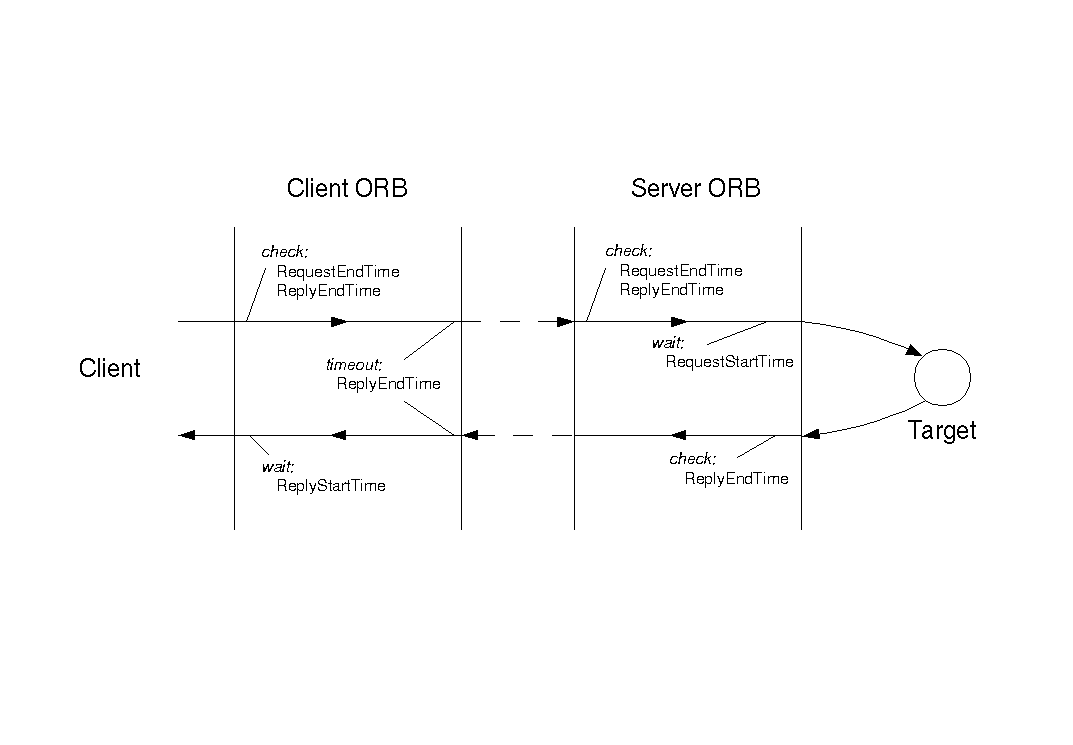
\includegraphics[width=16cm]{Timing.png}
  \end{center}
\caption{Timing Policies in JacORB}
\label{fig:timing}
\end{figure}

Figure \ref{fig:timing} shows how JacORB interprets the timing
policies in the course of a single request.  

\begin{itemize}
\item As soon as the ORB receives control (prior to marshalling), it
converts any \emph{RelativeRequestTimeoutPolicy} or
\emph{RelativeRoundtripTimeoutPolicy} to an absolute value, by adding
the relative value to the current system time.

\item The ORB then checks whether \emph{Request End Time} or
\emph{Reply End Time} have already elapsed.  If so, no invocation is
made, and an {\tt org.omg.CORBA.TIMEOUT} is thrown to the client.

\item After the ORB has sent the request, it waits for a reply until
\emph{Reply End Time} has elapsed.  If it receives no reply before
that, the request is discarded and an {\tt org.omg.CORBA.TIMEOUT}
thrown to the client.  (JacORB does not currently cancel the
outstanding request, it simply discards the reply, should one arrive
after the timeout has elapsed.)

\item On the server side (before demarshalling), the ORB checks
whether \emph{Request End Time} or \emph{Reply End Time} have already
elapsed.  If so, the request is not delivered to the target, and an
{\tt org.omg.CORBA.TIMEOUT} is thrown back to the client.

\item If the request proceeds, the ORB waits until the \emph{Reply
Start Time} has been reached, if one was specified, and has not
already elapsed.  After that, the request is delivered to the target.

\item After the target has returned control to the ORB, it checks
whether \emph{Reply End Time} has already elapsed.  If it has, the ORB
sends an {\tt org.omg.CORBA.TIMEOUT} back to the client, rather than
the actual reply.

\item If the reply arrives at the client before \emph{Reply End Time}
has elapsed, the ORB waits until \emph{Reply Start Time} has been
reached, if one was specified, and has not already elapsed.  After
that, the reply is delivered back to the client.

\end{itemize}

The bottom line of this is that for a simple, per-invocation timeout,
you should specify a \mbox{\emph{RelativeRoundtripTimeoutPolicy}}.  Note
that since this relative time is converted into an absolute time, and
also checked on the server side, the clocks on both the server and
the client need to be synchronized at least to the same order of
magnitude as the desired timeout.

\subsection*{Programming}

In CORBA, points of time are specified to an accuracy of 100~ns, using
values of struct {\tt TimeBase::UtcT}.  To allow easy manipulation of such
values from Java, JacORB provides a number of static methods in {\tt
org.jacorb.util.Time}.  For example, to convert the current Java time
into a {\tt UtcT} value, write

\begin{verbatim}
UtcT currentTime = org.jacorb.util.corbaTime();
\end{verbatim}

To create a {\tt UtcT} value that specifies a time $n$~ms in the
future, you can write

\begin{verbatim}
UtcT time = org.jacorb.util.corbaFuture (10000 * n);
\end{verbatim}

(The argument to {\tt corbaFuture()} is in CORBA time units of
100~ns; we multiply $n$ by 10000 here to convert it from Java time
units (milliseconds).)

The following shows how to set a timing policy for an object using the
standard mechanism (see the beginning of this chapter for an
explanation).  In this example, we set a \emph{Reply End Time} that
lies one second in the future:

\begin{verbatim}
import org.omg.CORBA.*;

SomeCorbaType server  = ...  // the object for which we want to set
                             // a timing policy
org.omg.CORBA.ORB orb = ...
org.omg.CORBA.Any a   = orb.create_any();

org.omg.TimeBase.UtcT replyEndTime 
    = org.jacorb.util.Time.corbaFuture (1000);  // one second

org.omg.TimeBase.UtcTHelper.insert (a, replyEndTime);

try
{
    Policy p 
        = orb.create_policy (REPLY_END_TIME_POLICY_TYPE.value, a);
    server._set_policy_override (new Policy[]{ p },
                                 SetOverrideType.ADD_OVERRIDE);
}
catch (PolicyError e)
{
    ...
}
\end{verbatim}

Using the constructors of JacORB's implementations of policy values,
this becomes less verbose:

\begin{verbatim}
SomeCorbaType server  = ...

Policy p = new org.jacorb.orb.policies.ReplyEndTimePolicy 
                         (org.jacorb.util.Time.corbaFuture (1000));

server._set_policy_override (new Policy[]{ p },
                             SetOverrideType.ADD_OVERRIDE);
\end{verbatim}

Likewise, to set a \emph{Relative Roundtrip Timeout} of one second,
write:

\begin{verbatim}
SomeCorbaType server  = ...

Policy p = 
    new org.jacorb.orb.policies.RelativeRoundtripTimeoutPolicy (1000);

server._set_policy_override (new Policy[]{ p },
                             SetOverrideType.ADD_OVERRIDE);
\end{verbatim}

The difference between this and the example before, where a
\emph{Reply End Time} was used, is that the latter specifies a
\emph{relative time} to CORBA.  The policy will therefore be valid
for all subsequent invocations, because the absolute deadline will be
recomputed before each invocation.  In the first example, the
deadline will no longer make sense for any subsequent invocations,
since only an absolute time was specified to the ORB.


%%%%%%%%%%%%%%%%%%%%%%%%%%%%%%%%%%%%%%%%%%%%%%%%%%%%%%%%%%%%%%%%%%%%%%%%%%%%%%

\chapter{Connection Management and Connection Timeouts}
\label{connection_management_timeouts}

JacORB offers a certain level of control over connections and timeouts. You
can 
\begin{itemize}
\item set connection idle timeouts.
\item set request timing. 
\item set the maximum number of accepted TCP/IP connections on the server.
\end{itemize}

\section{Timeouts}
\label{connection_timeouts}
Connection idle timeouts can be set individually for the client and the
server. They control how long an idle connection, i.e.~a connections that has
no pending replies, will stay open. The corresponding properties are {\tt
  jacorb.connection.client\_idle\_timeout} and {\tt
  jacorb. connection.server\_timeout} and take their values as microseconds. If
not set, connections will stay open indefinitely (or until the OS decides to
close them).

Request timing controls how long an individual request may take to
complete.  The programmer can specify this using QoS policies,
discussed in chapter \ref{qos}.

\section{Connection Management}
\label{connection_management}

When a client wants to invoke a remote object, it needs to send the request
over a connection to the server. If the connection isn't present, it has to be
created. In JacORB, this will only happen once for every combination of host
name and port. Once the connection is established, all requests and replies
between client and server will use the same connection. This saves resources
while adding a thin layer of necessary synchronization, and is the recommended
approach of the OMG. Occasionally people have requested to allow for multiple
connections to the same server, but nobody has yet presented a good argument
that more connections would speed up things considerably.

On the server side, the property {\tt
  jacorb.connection.max\_server\_transports} allows to set the maximum number
of TCP/IP connections that will be listened on for requests. When using a
network sniffer or tools like netstat, more inbound TCP/IP connections than
the configured number may be displayed. This is for the following reason:
Whenever the connection limit is reached, JacORB tries to close existing idle
connections (see the subsection below). This is done on the thread
that accepts the new connections, so JacORB will not actively accept more
connections. However, the ServerSocket is initialized with a backlog of 20.
This means that 20 more connections will be quasi-accepted by the OS. Only the
21st will be rejected right away.

\subsection{Basics and Design}
\label{connection_management_basics}
Whenever there is the need to close an existing connection because of the
connection limit, the question arises on which of the connection to close. To
allow for maximum flexibility, JacORB provides the interface {\tt
  SelectionStrategy} that allows for a custom way to select a connection to
close. Because selecting a connection usually requires some sort of
statistical data about it, the interface {\tt
  StatisticsProvider} allows to implement a class that collects statistical
data.

\begin{small}
\begin{verbatim}
package org.jacorb.orb.connection;

public interface SelectionStrategy
{
    public ServerGIOPConnection 
        selectForClose( java.util.List connections );
}

public interface StatisticsProvider 
{
    public void messageChunkSent( int size );
    public void flushed();
    public void messageReceived( int size );
}
\end{verbatim}
\end{small}

The interface {\tt SelectionStrategy} has only the single method of {\tt
  selectForClose()}. This is called by the class {\tt GIOPConnectionManager}
when a connection needs to be closed. The argument is a {\tt List} containing
objects of type {\tt ServerGIOPConnection}. The call itself is synchronized in
the {\tt GIOPConnectionManager}, so no additional synchronization has to be
done by the implementor of {\tt SelectionStrategy}. When examining the
connections, the strategy can get hold of the {\tt StatisticsProvider} via the
method {\tt getStatisticsProvider()} of the class {\tt GIOPConnection}. The
strategy implementor should take care only to return idle connections. While
the connection state is checked anyway while closing (it may have changed in
the meantime), it seems to be more efficient to avoid cycling through the
connections. When no suitable connection is available, the strategy may
return {\tt null}. The {\tt GIOPConnectionManager} will then wait for a
configurable time, and try again. This goes on until a connection can be
closed.
  
The interface {\tt StatisticsProvider} is used to collect statistical data
about a connection and provide it to the {\tt SelectionStrategy}.  Because the
nature of this data may vary, there is no standard access to the data via the
interface. Therefore, {\tt StatisticsProvider} and {\tt SelectionStrategy}
usually need to be implemented together. Whenever a new connection is
created\footnote{Currently, connection management is only implemented for the
  server side. Therefore, only accepted {\tt ServerGIOPConnections}s will get
  a {\tt StatisticsProvider}}, a new {\tt StatisticsProvider} object is
instanciated and stored with the {\tt Transport}\footnote{This is actually
  only done when a {\tt StatisticsProvider} is configured}. The {\tt
  StatisticsProvider} interface is oriented along the mode of use of the {\tt
  Transport}. For efficiency reasons, messages are not sent as one big byte
array. Instead, they are sent piecewise over the wire. When such a chunk is
sent, the method {\tt messageChunkSent(int size)} will be called. After the
message has been completely sent, method {\tt flush()} is called. This whole
process is synchronized, so all consecutive {\tt messageChunkSent}s until a
{\tt flush()} form a single message. Therefore, no synchronization on this
level is necessary. However, access to gathered statistical data by the {\tt
  SelectionStrategy} is concurrent, so care has to be taken. Receiving
messages is done only on the whole, so there exists only one method, {\tt
  messageReceived(int size)}, to notify the {\tt StatisticsProvider} of such
an event.

JacORB comes with two pre-implemented strategies: least frequently used and
least recently used. LFU and LRU are implemented by the classes {\tt
  org.jacorb.orb.con\-nection.L[F|R]USelectionStrategyImpl} and {\tt
  org.jacorb.orb.connection. L[F|R]U\-Statistics\-ProviderImpl}.

\subsection{Configuration}
\label{connection_management_config}
To configure connection management, the following properties are provided:
\begin{description}
\item {\tt jacorb.connection.max\_server\_transports} This property sets the
  maximum number of TCP/IP connections that will be listened on by the
  server--side ORB.
\item {\tt jacorb.connection.wait\_for\_idle\_interval} This property sets the
  interval to wait until the next try is made to find an idle connection to
  close. Value is in microseconds.
\item {\tt jacorb.connection.selection\_strategy\_class} This property sets
  the {\tt Selection\-Strategy}.
\item {\tt jacorb.connection.statistics\_provider\_class} This property sets
  the {\tt Statistics\-Provider}.
\item {\tt jacorb.connection.delay\_close} If turned on, JacORB will delay
  closing of TCP/IP connections to avoid certain situations, where message
  loss can occur. See also section \ref{connection_management_limitations}.
\end{description}

\subsection{Limitations}
\label{connection_management_limitations}
No sunshine without rain. When trying to close a connection, it is first
checked that the connection is idle, i.e.~has no pending messages.
If this is the case, a GIOP CloseConnection message is sent, and the
TCP/IP connection is closed. Under high load, this can lead to the following
situation:

\begin{enumerate}
\item Server sends the CloseConnection message.
\item Server closes the TCP/IP connection.
\item The client sends a new request into the connection, because it hasn't
  yet read and acted on the CloseConnection message.
\item The server--side OS will send a TCP RST, which cancels out the
  CloseConnection message.
\item The client finds the connection closed and must consider the request lost.
\end{enumerate}

To get by this situation, JacORB takes the following approach. Instead of
closing the connection right after sending the CloseConnection message, we
delay closing and wait for the client to close the connection. This behaviour
is turned off by default, but can be enabled by setting the property {\tt
  jacorb.connection.delay\_close} to ``yes''. When non-JacORB clients are used
care has to be taken that these ORBs do actively close the connection upon
receiving a CloseConnection message.

%%%%%%%%%%%%%%%%%%%%%%%%%%%%%%%%%%%%%%%%%%%%%%%%%%%%%%%%%%%%%%%%%%%%%%%%%%%%%%

\chapter{JacORB utilities}

In this chapter, we will briefly explain the executables that come
with JacORB. These include the IDL--compiler, the JacORB name server.


\section{idl}

The IDL compiler parses IDL specifications  and maps these to a set of
Java classes. IDL interfaces  are translated into Java interfaces, and
typedefs,   structs,   const  declarations   etc.   are  mapped   onto
corresponding Java  classes.  Using {\tt idl},  stubs and
skeletons  for  all interface  types  in  the  IDL specification  will
automatically be generated.

\subsection*{Usage}

\noindent{\tt idl
  [-h|-help] [-v|-version] [-syntax] [-all] [-Idir] [-Dsymbol[=value]]
  [-d <Output Dir>] [-p <package\_prefix>] [-i2jpackage <mapping>]
  [-W debug\_level] [-nofinal]   <filelist>}

The option {\tt  -v} prints out a short version  string while {\tt -h}
or {\tt -help} displays brief usage information.

The {\tt -noskel} option suppresses the generation of skeleton files,
which may be unnecessary if you only want to {\em use} a reference and
thus need client--side code.

The  {\tt -ir} option  instructs the  compiler to  generate additional
files   that    contain   information   needed    by   the   Interface
Repository. Basically, there  is one (very small) extra  file for each
IDL module, and another additional file per IDL interface.

Invoking {\tt idl}  with the {\tt -syntax} option  allows you to check
your IDL  specification for  syntactic errors without  producing code.
Without {\tt  -syntax}, the compiler creates  directories according to
the Java package structure.

The  compiler  does  not,  by  default,  generate  code  for  included
files. If that is desired, you have to use the {\tt -all} option which
causes code to be generated  for every IDL file directly or indirectly
included from within  {\tt <filelist>}. If you want  to make sure that
for a given IDL no code will  be generated even if this option is set,
you  can use  the  (proprietary) preprocessor  directive {\tt \#pragma
inhibit\_code\_generation}.

The {\tt-I} options allows you to specify one or more search paths for
IDL files included from within  {\tt <filelist>}. If no path is given,
only the  current directory will  be considered.

With the  {\tt -D} option you can  define symbols that can  be used by
the  preprocessor while  processing  the  IDL file.   If  no value  is
specified, the  symbol will be  defined with a  value of 1. The {\tt
  -U} option lets you undefine symbols again.

Compiling a  file with  a module {\tt  ModuleX} and an  interface {\tt
  InterfaceY} in it  will result in a subdirectory  {\tt ModuleX} with
  {\tt    InterfaceY.java}   in   it    (and   possibly    more   {\tt
  .java}--files). By default, the root  directory for all of the files
  created  during  the process  is  the  current  directory. You  can,
  however, provide a  different directory in which these  files are to
  be placed by  using the -d option. Using the -d  option when you are
  only checking the syntax of an IDL file has no effect.

By using the {\tt -nofinal} option the compiler can be made to generate
class definitions that are not final. This will override the default
behaviour, which is to generate final class definitions in certain
circumstances to allow for their optimisation during compilation.

With the  {\tt -p}  option it  is also possible  to specify  a package
prefix for the generated Java  classes. E.g., if the IDL file contains
a module {\tt Bank} which  defines an interface {\tt Account}, you can
direct   the   IDL   compiler    to   generate   Java   classes   {\tt
example.Bank.Account} by compiling with the package prefix set to {\tt
example}, i.e. by compiling with

\cmdline{idl -p example bank.idl}

The IDL compiler will create the appropriate directories if necessary.
Note that the effect is the same as if the entire contents of the IDL
file was scoped with {\tt example}. In particular, this applies to
included files: all definitions in included files will also be scoped
this way! The -p switch should used with discretion in cases where
other IDL files are included.

To be able to flexibly redirect generated Java classes into packages,
the {\tt -i2jpackage} switch can be used. Using this option, any IDL
scope x can be replaced by one (or more) Java packages y. Specifying
{\tt -i2jpackage X:a.b.c} will thus cause code generated for IDL
definitions within a scope x to end up in a Java package {\tt a.b.c},
e.g. an IDL identifier {\tt X::Y::ident} will be mapped to {\tt
  a.b.c.y.ident} in Java.

(The  IDL  parser  was   generated  with  Scott  Hudson's  CUP  parser
generator.  The  LALR grammar for  the CORBA IDL  is in the  file {\tt
jacorb/Idl/parser.cup}.)

\section{ns}

JacORB provides a service for mapping names to network references. The
name server itself is written in Java like the rest of the package and
is a  straightforward implementation  of the CORBA  ``Naming Service''
from  Common  Object Services  Spec.,  Vol.1  \cite{OMG1997}. The  IDL
interfaces are mapped to Java according to our Java mapping.

\subsection*{Usage}

\cmdline{ns <filename>  [<timeout>]}

or

\cmdline{jaco jacorb.Naming.NameServer <filename>  [<timeout>]}

\subsection*{Example}

\cmdline{ns \~/public\_html/NS\_Ref}

The name server does {\it not}  use a well known port for its service.
Since clients  cannot (and  need not) know  in advance where  the name
service will  be provided, we use  a bootstrap file in  which the name
server records  an object reference to itself  (its {\it Interoperable
Object Reference} or  IOR). The name of this bootstrap  file has to be
given as an argument to the  {\tt ns} command. This bootstrap file has
to  be available  to clients  network-wide, so  we demand  that  it be
reachable  via a  URL  --- that  is,  there must  be an  appropriately
configured HTTP server in your network domain which allows read access
to the bootstrap  file over a HTTP connection.  (This implies that the
file must have its read  permissions set appropriately. If the binding
to the name service fails, please  check that this is the case.) After
locating the name service through this mechanism, clients will connect
to the name server directly, so the only HTTP overhead is in the first
lookup of the server.

The name bindings in the server's database are stored in and retrieved
from a file that is found in the current directory unless the property
{\tt jacorb.naming.db\_dir} is set to a different directory name. When
the server  starts up, it tries  to read this file's  contents. If the
file  is  empty or  corrupt,  it will  be  ignored  (but overridden  on
exit). The name server can only save its state when it goes down after
a specified timeout. If the server is interrupted (with {\tt CTRL-C}),
state information  is lost  and the file  will not contain  any usable
data.

If no timeout is specified, the name server will simply stay up until
it is killed. Timeouts are specified in milliseconds.

\section{nmg}

The JacORB  NameManager, a  GUI for the  name service, can  be started
using the {\tt nmg} command.  The NameManager then tries to connect to
an existing name service.

\subsection*{Usage}

\cmdline{nmg}

\section{lsns}

This utility  lists the contents  of the default naming  context. Only
currently active servers that have registered are listed. The {\tt -r}
option recursively lists the  contents of naming contexts contained in
the root  context. If  the graph of  naming contexts  contains cycles,
trying to list the entire contents recursively will not return...

\subsection*{Usage}


\cmdline{lsns [-r] }

\subsection*{Example}

\cmdline{lsns \\
\ /grid.service}

when only the server for the grid example is running and registered
with the name server.


\section{dior}

JacORB comes with a simple utility to decode an interoperable object reference
(IOR) in string form into a more readable representation.

\subsection*{Usage}

\cmdline{dior <IOR-string> | -f <filename>}

\subsection*{Example}

In the following example we use it to print out the contents of the
IOR that the JacORB name server writes to its file:

\cmdline{dior -f \~/public\_html/NS\_Ref}
\small{\begin{verbatim}
------IOR components-----
TypeId  :       IDL:omg.org/CosNaming/NamingContextExt:1.0
Profile Id   :  TAG_INTERNET_IOP
IIOP Version :  1.0
Host    :       160.45.110.41
Port    :       49435
Object key :    0x52 6F 6F 74 50 4F 41 3A 3A 30 D7 D1 91 E1 70 95 04
\end{verbatim}
}

\section{pingo}

``Ping'' an object using its stringified IOR. Pingo will call {\tt
  \_non\_existent()} on the object's reference to determine whether
  the object is alive or not.

\subsection*{Usage}

\cmdline{pingo <IOR-string> | -f <filename> }

\section{ir}

This command starts the JacORB Interface Repository, which is explained in
chapter \ref{ch:interface_repository}.

\subsection*{Usage}

\cmdline{ir <reppository class path> <IOR filename> }

\section{qir}

This command queries the JacORB Interface Repository and prints out
re--generated IDL for the repository item denoted by the argument
repository ID.

\subsection*{Usage}

\cmdline{qir <reppository Id> }

\section{ks}

This command starts the JacORB KeyStoreManager, which is explained in
chapter \ref{SSL}

\subsection*{Usage}

\cmdline{ks}

\section{fixior}

This command patches host and port information into an IOR file.

\subsection*{Usage}

\cmdline{fixior <host> <port> <ior\_file> }

%%%%%%%%%%%%%%%%%%%%%%%%%%%%%%%%%%%%%%%%%%%%%%%%%%%%%%%%%%%%%%%%%%%%%%%%%%%%%%
\chapter{Configuration Properties}

A comprehensive listing and description of the properties which are used
to configure JacORB are given in the following tables.

\begin{small}
\begin{longtable}{|p{5cm}|p{9cm}|p{2cm}|}
\caption{ORB Configuration}\\
\hline
~ \hfill \textbf {Property} \hfill ~ & ~ \hfill \textbf {Description} \hfill ~ & ~ \hfill \textbf {Type} \hfill ~ \endhead
\hline
\verb"ORBInitRef.<service>" & Properties of this form configure initial service objects which can be resolved via the ORB resolve\_initial\_references. A variety of URL formats are supported. & URL \\
\hline
\verb"org.omg.PortableInterc"
\verb"eptor.ORBInitializerCl"
\verb"ass.<name>" & A portable interceptor initializer class instantiated at ORB creation. & class \\
\hline
\verb"jacorb.orb.objectKeyMa"
\verb"p.<name>" & Maps an object key to an arbitrary string thereby enabling better readability for corbaloc URLs. & string \\
\hline
\verb"jacorb.orb.print_versi"
\verb"on" & If enabled, the ORB's version number is printed whenever the ORB is initialized. Default is on. & boolean \\
\hline
\verb"jacorb.verbosity" & Diagnostic verbosity level: 0 = off, 1 = important messages and exceptions,  $>$= 3 = debug-level output (output may be extensive) & integer \\
\hline
\verb"jacorb.logfile" & Output destination for diagnostic log file. If not set, then diagnostics are sent to standard output. & file \\
\hline
\verb"jacorb.logfile.append" & If logging to file whether to append to existing file or overwrite. Default is off. & boolean \\
\hline
\verb"jacorb.logfile.maxLogS"
\verb"ize" & If appending to a file sets the size in kilobytes at which the file is rolled over. Default is off (0). & integer \\
\hline
\verb"jacorb.log.timestamp" & Whether to timestamp log messages. Default is off & boolean \\
\hline
\verb"jacorb.debug.dump_outg"
\verb"oing_messages" & Hex dump outgoing messages. Default is off. & boolean \\
\hline
\verb"jacorb.debug.dump_inco"
\verb"ming_messages" & Hex dump incoming messages. Default is off. & boolean \\
\hline
\verb"jacorb.giop_minor_vers"
\verb"ion" & The GIOP minor version number to use for newly created IORs. Default is 2. & integer \\
\hline
\verb"jacorb.retries" & Number of retries if connection cannot directly be established. Default is 5. & integer \\
\hline
\verb"jacorb.retry_interval" & Time in milliseconds to wait between retries. Default is 500. & millisec. \\
\hline
\verb"jacorb.outbuf_size" & Size of network buffers for outgoing messages in bytes. Default is 2048. & byte \\
\hline
\verb"jacorb.maxManagedBufSi"
\verb"ze" & This is NOT the maximum buffer size that can be used, but just the largest size of buffers that will be kept and managed. This value will be added to an internal constant of 5, so the real value in bytes is 2** (5 + maxManagedBufSize - 1). You only need to increase this value if you are dealing with LOTS of LARGE data structures. You may decrease it to make the buffer manager release large buffers immediately rather than keeping them for later reuse. Default is 18. & integer \\
\hline
\verb"jacorb.connection.clie"
\verb"nt_timeout" & Client-side timeout. This is set to non-zero in order to stop blocking after specified number of milliseconds. Not set by default. & millisec. \\
\hline
\verb"jacorb.connection.serv"
\verb"er_timeout" & Maximum time in milliseconds that a server keeps a connection open if nothing happens. Not set by default. & millisec. \\
\hline
\verb"jacorb.connection.max"
\verb"_server_transports" & This property sets the
  maximum number of TCP/IP connections that will be listened on by the
  server--side ORB. Default is unlimited connections & integer \\
\hline
\verb"jacorb.connection.wait"
\verb"_for_idle_interval" & This property sets the
  interval to wait until the next try is made to find an idle connection to
  close. Default is 500 & millisec.\\
\hline
\verb"jacorb.connection.sele"
\verb"ction_strategy_class" & This property sets
  the {\tt Selection\-Strategy} & class \\
\hline
\verb"jacorb.connection.stat"
\verb"istics_provider_class" & This property sets
  the {\tt Statistics\-Provider} & class \\
\hline
\verb"jacorb.connection.del"
\verb"ay_close" & This property controls the behaviour after sending a GIOP
CloseConnection messsage. If set to ``on'', the TCP/IP connection won't be
closed directly. Instead, it is waited for the client to do so first. Default is off. & boolean \\
\hline
\verb"jacorb.reference_cachi"
\verb"ng" & Whether or not JacORB caches objects references. Not set by default. & boolean \\
\hline
\verb"jacorb.hashtable_class" & The following property specifies the class which is used for reference caching. WeakHashtable uses WeakReferences, so entries get garbage collected if only the Hashtable has a reference to them. This is useful if you have many references to short-living non-persistent CORBA objects. It is only available for java 1.2 and above. On the other hand the standard Hashtable keeps the references until they are explicitly deleted by calling \_release(). This is useful for persistent and long-living CORBA objects. Defaults to Hashtable. & class \\
\hline
\verb"jacorb.use_bom" & Use GIOP 1.2 byte order markers, since CORBA 2.4-5. Default is off. & boolean \\
\hline
\verb"jacorb.giop.add_1_0_pr"
\verb"ofiles" & Add additional IIOP 1.0 profiles even if using IIOP 1.2. Default is off. & boolean \\
\hline
\verb"jacorb.dns.enable" & Use DNS when DNS support has been included in build. Default is on. & boolean \\
\hline
\verb"org.omg.PortableInterc"
\verb"eptor.ORBInitializerCl"
\verb"ass.bidir_init" & This portable interceptor must be configured to support bi-directional GIOP. Not set by default. & class \\
\hline
\verb"jacorb.ior_proxy_host" & The jacorb.ior\_proxy\_host and jacorb.ior\_proxy\_port properties inform the ORB what IP/port IORs should contain, if the ServerSockets IP/port can't be used (e.g. for traffic through a firewall). WARNING: this is just �dumb� replacing, so you have to take care of your configuration! Not set by default. & node \\
\hline
\verb"jacorb.ior_proxy_port" & See jacorb.ior\_proxy\_host above. Not set by default. & port \\
\hline
\verb"OAIAddr" & The Object Adapter Internet Address: IP address on multi-homed host (this gets encoded in object references). NOTE: Addresses like 127.0.0.X will only be accessible from the same machine! Not set by default. & node \\
\hline
\verb"OAPort" & See OAIAddr above. Not set by default. & port \\
\hline
\verb"org.omg.PortableInterc"
\verb"eptor.ORBInitializerCl"
\verb"ass.standard_init" & Standard portable interceptor. DO NOT REMOVE. & class \\
\hline
\verb"jacorb.net.socket_fact"
\verb"ory" & Sets or defines the socket factory that must implement the operations defined in the org.jacorb.orb.factory.SocketFactory interface. & class \\
\hline
\verb"jacorb.net.server_sock"
\verb"et_factory" & Sets or defines the socket factory that must implement the operations defined in the org.jacorb.orb.factory.ServerSocketFactory interface. & class \\
\hline
\verb"jacorb.net.socket_fact"
\verb"ory.port.min" & Sets the minimum port number that can be used for an additional supported socket factory. This property is used in conjunction with the jacorb.net.socket\_factory.port.max property. These properties enable the factory to traverse firewalls through a fixed port range. Default is unset, disabling the factory. & integer \\
\hline
\verb"jacorb.net.socket_fact"
\verb"ory.port.max" & Sets the maximum port number that can be used for the additional supported socket factory. Refer to jacorb.net.socket\_factory.port.min above. Default is unset, disabling the factory. & integer \\
\hline

\end{longtable}
\end{small}


\begin{small}
\begin{longtable}{|p{5cm}|p{9cm}|p{2cm}|}
\caption{Appligator Configuration}\\
\hline
~ \hfill \textbf {Property} \hfill ~ & ~ \hfill \textbf {Description} \hfill ~ & ~ \hfill \textbf {Type} \hfill ~ \endhead
\hline
\verb"jacorb.ProxyServer.URL" & This is the URL for the default Appligator and is used when applets or firewall traversal is supported via the JacORB Appligator.  & URL \\
\hline
\verb"jacorb.ProxyServer.URL"
\verb"-<network>-<netmask>" & Additional appligators can be configured for remote subnets using this subnet form of URL configuration. The subnet for a scoped appligator is calculated by the logical ANDing of the network and netmask values.  & URL \\
\hline
\verb"jacorb.ProxyServer.Nam"
\verb"e" & The name the appligator uses when adding itself to the Name Service (if available) on start up. Default is Appligator. & string \\
\hline
\verb"jacorb.ProxyServer.ID" & Defines the object identity for the appligator IOR. If not set, then this defaults to 'Appligator': it is recommended that this is set to some other value for additional security. & string \\
\hline
\verb"jacorb.ProxyServer.Net"
\verb"mask" & Optionally used to configure the network for the local client. When used, the calls to objects within the local subnet will not be redirected. Not set by default. & IP address \\
\hline
\verb"jacorb.ProxyServer.Net"
\verb"work" & See jacorb.ProxyServer.Netmask above. Not set by default. & IP address \\
\hline

\end{longtable}
\end{small}


\begin{small}
\begin{longtable}{|p{5cm}|p{9cm}|p{2cm}|}
\caption{POA Configuration}\\
\hline
~ \hfill \textbf {Property} \hfill ~ & ~ \hfill \textbf {Description} \hfill ~ & ~ \hfill \textbf {Type} \hfill ~ \endhead
\hline
\verb"jacorb.poa.monitoring" & Displays a GUI monitoring tool for servers. Default is off. & boolean \\
\hline
\verb"jacorb.poa.thread_pool"
\verb"_max" & Maximum thread pool configuration for request processing & integer \\
\hline
\verb"jacorb.poa.thread_pool"
\verb"_min" & Minimum thread pool configuration for request processing & integer \\
\hline
\verb"jacorb.poa.thread_prio"
\verb"rity" & If set, request processing threads in the POA will run at this priority. If not set or invalid, MAX\_PRIORITY will be used. Not set by default. & integer \\
\hline
\verb"jacorb.poa.queue_max" & The size of the request queue. Clients will receive Corba.TRANSIENT exceptions if load exceeds this limit. Default is 100. & integer \\
\hline

\end{longtable}
\end{small}


\begin{small}
\begin{longtable}{|p{5cm}|p{9cm}|p{2cm}|}
\caption{Implementation Repository Configuration}\\
\hline
~ \hfill \textbf {Property} \hfill ~ & ~ \hfill \textbf {Description} \hfill ~ & ~ \hfill \textbf {Type} \hfill ~ \endhead
\hline
\verb"jacorb.use_imr" & Switch on to contact the Implementation Repository (IR) on every server start-up. Default is off. & boolean \\
\hline
\verb"jacorb.use_imr_endpoin"
\verb"t" & Switch off to prevent writing the IMR address into server IORs. This property is ignored if jacorb.use\_imr = off. Default is off. & boolean \\
\hline
\verb"jacorb.imr.allow_auto_"
\verb"register" & If set to on servers that don't already have an entry on their first call to the IR, will get automatically registered. Otherwise, an UnknownServer exception is thrown. Default is off. & boolean \\
\hline
\verb"jacorb.imr.check_objec"
\verb"t_liveness" & If set on the IR will try to ping every object reference that it is going to return. If the reference is not alive, then TRANSIENT is thrown. Default is off. & boolean \\
\hline
\verb"ORBInitRef.Implementat"
\verb"ionRepository" & The initial reference for the IR. & URL \\
\hline
\verb"jacorb.imr.table_file" & File in which the IR stores data. & file \\
\hline
\verb"jacorb.imr.backup_file" & Backup data file for the IR. & file \\
\hline
\verb"jacorb.imr.ior_file" & File to which the IR writes its IOR. This is usually referred to by the initial reference for the IR (configured above).  & file \\
\hline
\verb"jacorb.imr.timeout" & Time in milliseconds that the implementation will wait for a started server to register. After this timeout is exceeded the IR assumes the server has failed to start. Default is 12000 (2 minutes). & millisec. \\
\hline
\verb"jacorb.imr.no_of_poas" & Initial number of POAs that can be registered with the IR. This is an optimization used to size internal data structures. This value can be exceeded. Default is 100. & integer \\
\hline
\verb"jacorb.imr.no_of_serve"
\verb"rs" & Initial number of servers that can be registered with the IR. This is an optimization used to size internal data structures. This value can be exceeded. Default is 5. & integer \\
\hline
\verb"jacorb.imr.port_number" & Starts the IMR on a fixed port (equivalent to the -p option). & integer \\
\hline
\verb"jacorb.imr.connection_"
\verb"timeout" & Time in milliseconds that the IR waits until a connection from an application client is terminated. Default is 2000. & millisec. \\
\hline
\verb"jacorb.implname" & The implementation name for persistent servers. Persistent servers should set this to a unique name. This is the service name that is registered in the IR. & name \\
\hline
\verb"jacorb.java_exec" & Command used by the IR to start servers. & command \\
\hline

\end{longtable}
\end{small}


\begin{small}
\begin{longtable}{|p{5cm}|p{9cm}|p{2cm}|}
\caption{Security Configuration}\\
\hline
~ \hfill \textbf {Property} \hfill ~ & ~ \hfill \textbf {Description} \hfill ~ & ~ \hfill \textbf {Type} \hfill ~ \endhead
\hline
\verb"OASSLPort" & The port number used by SSL, will be dynamically assigned by default. & port \\
\hline
\verb"org.omg.PortableInterc"
\verb"eptor.ORBInitializerCl"
\verb"ass.ForwardInit" & Portable interceptor required to support SSL. Not set by default. & class \\
\hline
\verb"jacorb.security.access"
\verb"_decision" & The qualified classname of access decision object. & class \\
\hline
\verb"jacorb.security.princi"
\verb"pal_authenticator" & A list of qualified classnames of principle authenticator objects, separated by commas (no whitespaces.). The first entry (that can be successfully created) will be available through the principal\_authenticator property. & class \\
\hline
\verb"jacorb.ssl.socket_fact"
\verb"ory" & The qualified classname of the SSL socket factory class. & class \\
\hline
\verb"jacorb.ssl.server_sock"
\verb"et_factory" & The qualified classname of the SSL server socket factory class. & class \\
\hline
\verb"jacorb.security.change"
\verb"_ssl_roles" & Exchange SSL client server roles to enforce client authentication. Beware: this causes problems with peers that not prepared to handle this role change. Default is off. & boolean \\
\hline
\verb"jacorb.security.suppor"
\verb"t_ssl" & Whether SSL security is supported. Default is off. & boolean \\
\hline
\verb"jacorb.security.ssl.cl"
\verb"ient.supported_options" & SSL client supported options - IIOP/SSL parameters (numbers are hex values, without the leading 0x): NoProtection = 1, EstablishTrustInClient = 40, EstablishTrustInTarget = 20, mutual authentication = 60. Default is 0. Please see the programming guide for more explanation. & integer \\
\hline
\verb"jacorb.security.ssl.cl"
\verb"ient.required_options" & SSL client required options (See IIOP/SSL parameters above). Default is 0. & integer \\
\hline
\verb"jacorb.security.ssl.se"
\verb"rver.supported_options" & SSL server supported options (See IIOP/SSL parameters above). Default is 0. & integer \\
\hline
\verb"jacorb.security.ssl.se"
\verb"rver.required_options" & SSL server required options (See IIOP/SSL parameters above). Default is 0. & integer \\
\hline
\verb"jacorb.security.ssl.co"
\verb"rbaloc_ssliop.supporte"
\verb"d_options" & Used in conjunction with jacorb.security.ssl.corbaloc\_ssliop.required\_options. If these properties are set, then two values will be placed in the IOR, "corbaloc:ssliop� and "ssliop�. If not set, only EstablishTrustInTarget is used for both supported and required options. & integer \\
\hline
\verb"jacorb.security.ssl.co"
\verb"rbaloc_ssliop.required"
\verb"_options" &  Default is 0. & integer \\
\hline
\verb"jacorb.security.keysto"
\verb"re" & The name and location of the keystore. This may be absolute or relative to the home directory. NOTE (for Sun JSSE users): The javax.net.ssl.trustStore [Password] properties doesn't seem to take effect, so you may want to add trusted certificates to normal keystores. In this case, please set the property jacorb.security.jsse. trustees\_from\_ks to on, so trusted certificates are taken from the keystore instead of a dedicated truststore.  & file \\
\hline
\verb"jacorb.security.keysto"
\verb"re_password" & The keystore password. & string \\
\hline
\verb"jacorb.security.truste"
\verb"es" & Files with public key certificates of trusted Certificate Authorities (CA). WARNING: If no CA certificates are present, the IAIK chain verifier will accept ALL otherwise valid chains. & file \\
\hline
\verb"jacorb.security.defaul"
\verb"t_user" & The name of the default key alias to look up in the keystore. & name \\
\hline
\verb"jacorb.security.defaul"
\verb"t_password" & The name of the default key alias to look up in the keystore. & string \\
\hline
\verb"jacorb.security.iaik_d"
\verb"ebug" & Sets IAIKS SSL classes to print debug output to standard output. Default is off. & boolean \\
\hline
\verb"jacorb.security.jsse.t"
\verb"rustees_from_ks" & Sun JSSE specific settings: Use the keystore to take trusted certificates from. Default is off. & boolean \\
\hline
\verb"jacorb.security.ssl.se"
\verb"rver.cipher_suites" & A comma-separated list of cipher suite names which must NOT contain whitespaces. See the JSSE documents on how to obtain the correct cipher suite strings. & string \\
\hline
\verb"jacorb.security.ssl.cl"
\verb"ient.cipher_suites" & See jacorb.security.ssl.server.cipher\_suites above. & string \\
\hline

\end{longtable}
\end{small}

%%%%%%%%%%%%%%%%%%%%%%%%%%%%%%%%%%%%%%%%%%%%%%%%%%%%%%%%%%%%%%%%%%%%%%%%%%%%%%

\chapter{Limitations, Feedback}

A few limitations and known bugs (list is incomplete):

\begin{itemize}
    \item the IDL compiler does not support
    \begin{itemize}
        \item the {\tt context} construct
    \end{itemize}
    \item the API documentation and this document are incomplete.
\end{itemize}

\subsection*{Feedback and bug reports}

For bug reporting, please use our Bugzilla bugtracking database available at
\href{http://www.jacorb.org/bugzilla}{http://www.jacorb.org/bugzilla}.  Please
send problems as well as criticism and experience reports to our developer
mailing list available from
\href{http://www.jacorb.org/contact.html}{http://www.jacorb.org/contact.html}.

%%%%%%%%%%%%%%%%%%%%%%%%%%%%%%%%%%%
{
\bibliography{./guide}
\bibliographystyle{alpha}
}

\end{document}
